%%%%%%%%%%%%%%%%%%%%%%%%%%%%%%%%%%%%%%%%%
% Beamer Presentation
% LaTeX Template
% Version 1.0 (10/11/12)
%
% This template has been downloaded from:
% http://www.LaTeXTemplates.com
%
% License:
% CC BY-NC-SA 3.0 (http://creativecommons.org/licenses/by-nc-sa/3.0/)
%
%%%%%%%%%%%%%%%%%%%%%%%%%%%%%%%%%%%%%%%%%

%----------------------------------------------------------------------------------------
%	PACKAGES AND THEMES
%----------------------------------------------------------------------------------------

\documentclass{beamer}

\mode<presentation> {

% The Beamer class comes with a number of default slide themes
% which change the colors and layouts of slides. Below this is a list
% of all the themes, uncomment each in turn to see what they look like.

%\usetheme{default}
%\usetheme{AnnArbor}
%\usetheme{Antibes}
%\usetheme{Bergen}
%\usetheme{Berkeley}
%\usetheme{Berlin}
%\usetheme{Boadilla}
%\usetheme{CambridgeUS}
%\usetheme{Copenhagen}
%\usetheme{Darmstadt}
%\usetheme{Dresden}
%\usetheme{Frankfurt}
%\usetheme{Goettingen}
%\usetheme{Hannover}
%\usetheme{Ilmenau}
%\usetheme{JuanLesPins}
%\usetheme{Luebeck}
%\usetheme{Madrid}
%\usetheme{Malmoe}
%\usetheme{Marburg}
%\usetheme{Montpellier}
%\usetheme{PaloAlto}
\usetheme{Pittsburgh}
%\usetheme{Rochester}
%\usetheme{Singapore}
%\usetheme{Szeged}
%\usetheme{Warsaw}

% As well as themes, the Beamer class has a number of color themes
% for any slide theme. Uncomment each of these in turn to see how it
% changes the colors of your current slide theme.

%\usecolortheme{albatross}
\usecolortheme{beaver}
%\usecolortheme{beetle}
%\usecolortheme{crane}
%\usecolortheme{dolphin}
%\usecolortheme{dove}
%\usecolortheme{fly}
%\usecolortheme{lily}
%\usecolortheme{orchid}
%\usecolortheme{rose}
%\usecolortheme{seagull}
%\usecolortheme{seahorse}
%\usecolortheme{whale}
%\usecolortheme{wolverine}

%\setbeamertemplate{footline} % To remove the footer line in all slides uncomment this line
%\setbeamertemplate{footline}[page number] % To replace the footer line in all slides with a simple slide count uncomment this line

%\setbeamertemplate{navigation symbols}{} % To remove the navigation symbols from the bottom of all slides uncomment this line
}
\usepackage{graphicx} % Allows including images
\usepackage{booktabs} % Allows the use of \toprule, \midrule and \bottomrule in tables

\usepackage{fontspec}
\setsansfont{Calibri}[
    Path=Font/,
    Scale=0.9,
    Extension = .ttf,
    UprightFont=*-Regular,
    BoldFont=*-Bold,
    ItalicFont=*-Italic,
    BoldItalicFont=*-BoldItalic
    ]
\usepackage{unicode-math}
\setmathfont{Libertinus Math}% 使用默认的数学字体或你偏好的数学字体 Latin Modern Math/Libertinus Math
% \setmathfont[version=bold]{Latin Modern Math}

\usepackage{tikz}
\usetikzlibrary{positioning}
\usetikzlibrary{calc}
\usepackage{ragged2e}
\justifying\let\raggedright\justifying %两端对齐
%----------------------------------------------------------------------------------------
%	TITLE PAGE
%----------------------------------------------------------------------------------------

\title[Asset Pricing]{\textbf{Asset Pricing}} % The short title appears at the bottom of every slide, the full title is only on the title page

\subtitle{6. Production-Based Asset Pricing}

\author[Cheng Hang]{Cheng Hang} % Your name
\institute[DUFE] % Your institution as it will appear on the bottom of every slide, may be shorthand to save space
{School of Fintech \\
Dongbei University of Finance \& Economics \\ % Your institution for the title page
\medskip
\textbf{chenghangch@qq.com}% Your email address
}
\date{\today} % Date, can be changed to a custom date

	\AtBeginSection[]
{
	\begin{frame}[allowframebreaks]{Content}
		\small
		\tableofcontents[sectionstyle=show/shaded,subsectionstyle=show/shaded/hide] %这几个参数我也不知道该如何准确地解释，反正它们最终的效果是突出显示当前章节，而其它章节都进行了淡化处理
		\addtocounter{framenumber}{-1}  %目录页不计算页码
	\end{frame}
}

%----------------------------------------------------------------------------------------
%	Begin
%----------------------------------------------------------------------------------------

\begin{document}

\begin{frame}
\titlepage % Print the title page as the first slide
\end{frame}

%\begin{frame}
%\frametitle{Overview} % Table of contents slide, comment this block out to remove it
%\tableofcontents % Throughout your presentation, if you choose to use \section{} and \subsection{} commands, these will automatically be printed on this slide as an overview of your presentation
%\end{frame}

%--------------------------------------
%	PRESENTATION SLIDES
%--------------------------------------

% ---------------------------------------------------------
% Roadmap: where Lecture 06 sits in the 3-act story
% ---------------------------------------------------------
\begin{frame}{Roadmap: From CAPM to Factor War}
	This lecture is \textbf{Act II} of a three-lecture arc.
	\vspace{4pt}
	\begin{center}
		\small
		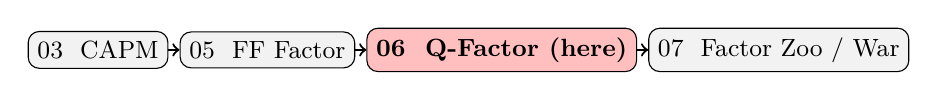
\begin{tikzpicture}[node distance=4pt, every node/.style={font=\small}]
			\node[draw,rounded corners,fill=gray!10] (a) {03~~CAPM};
			\node[draw,rounded corners,fill=gray!10,right=of a] (b) {05~~FF Factor};
			\node[draw,rounded corners,fill=red!25,right=of b] (c) {\textbf{06~~Q-Factor (here)}};
			\node[draw,rounded corners,fill=gray!10,right=of c] (d) {07~~Factor Zoo / War};
			\draw[->,thick] (a) -- (b);
			\draw[->,thick] (b) -- (c);
			\draw[->,thick] (c) -- (d);
		\end{tikzpicture}
	\end{center}

\href{https://theinvestmentcapm.com/index.html}{\textcolor{blue}{Zhang Lu's Website: Investment CAPM}}    

\end{frame}

% ---------------------------------------------------------
% Recap: where Lecture 05 left off
% ---------------------------------------------------------
\begin{frame}{Where We Left Off}
	Lecture 05 ended with a clean problem statement:
	\begin{itemize}
		\item FF3 cannot price four large anomalies: \textbf{momentum, profitability, investment, IVOL}.
		\item Two repair routes emerged:
		\begin{itemize}
			\item \textit{Empirical patch}: keep adding factors $\rightarrow$ Carhart (1997), \href{https://doi.org/10.1016/j.jfineco.2014.10.010}{\textcolor{blue}{FF5 (2015)}}, \href{https://doi.org/10.1016/j.jfineco.2018.02.012}{\textcolor{blue}{FF6 (2018)}}.
			\item \textit{Theoretical reset}: derive factors from a structural model.
		\end{itemize}
	\end{itemize}
	\vspace{4pt}
	\begin{block}{This lecture takes Route 2 seriously}
		Starting from the firm's investment first-order condition (\textit{q}-theory), we derive a model in which \textbf{investment} ($I/A$) and \textbf{profitability} (ROE) must price the cross-section. The deliverable is the \href{https://doi.org/10.1093/rfs/hhu068}{\textcolor{blue}{Hou-Xue-Zhang (2015) \textit{q}-factor model}}, the most prominent rival to FF5.
	\end{block}
\end{frame}

% ---------------------------------------------------------
% Narrative spine: what problem each block solves
% ---------------------------------------------------------
\begin{frame}{The Narrative: Four Locks}
	\small
	The lecture is not a list of q-theory results. It opens four locks in sequence:
	\vspace{4pt}
	\begin{enumerate}
		\item \textbf{Legitimacy:} Can factors be \textit{derived} from firm optimization rather than mined from anomalies?
		\item \textbf{Measurement:} The FOC gives marginal $q$; under CRS, can we replace it with observable average $q$?
		\item \textbf{Return bridge:} Can accounting variables imply returns without specifying household preferences?
		\item \textbf{Empirical weapon:} Can investment and profitability become a traded factor model that challenges FF5?
	\end{enumerate}
	\vspace{4pt}
	\begin{block}{How to read the math}
		Equations in Sections 1--5 \textbf{build the machine}; Sections 6--12 turn that machine into \textbf{testable returns and factors}.
	\end{block}
\end{frame}

% ---------------------------------------------------------
% Two paradigms side-by-side
% ---------------------------------------------------------
\begin{frame}{Two Paradigms of Asset Pricing}
	\small
	\begin{tabular}{@{}p{0.46\linewidth}p{0.46\linewidth}@{}}
		\toprule
		\textbf{Demand side (consumption-based)} & \textbf{Supply side (production-based)} \\
		\midrule
		Investor's Euler equation: \par $1 = \mathrm{E}_t[M_{t+1}R_{t+1}]$. & Firm's investment Euler equation: \par $1 = \mathrm{E}_t[M_{t+1} R^I_{t+1}]$. \\
		\addlinespace
		Pricing kernel from \textbf{marginal utility of consumption} or empirical mimicking portfolios. & Pricing kernel disciplined by \textbf{marginal cost / marginal benefit of investment}. \\
		\addlinespace
		Headline models: CCAPM, ICAPM, FF3, FF5, FF6. & Headline models: \href{https://doi.org/10.1111/j.1540-6261.1991.tb03750.x}{\textcolor{blue}{Cochrane (1991)}}, \href{https://doi.org/10.1086/649760}{\textcolor{blue}{LWZ (2009)}}, \href{https://doi.org/10.1093/rfs/hhu068}{\textcolor{blue}{HXZ (2015) $q$}}, HMXZ (2021) $q^5$. \\
		\addlinespace
		Factors are constructed \textit{ex post} from anomaly portfolios. & Factors are dictated \textit{ex ante} by the firm's first-order conditions. \\
		\addlinespace
		Strength: flexible, easy to extend. & Strength: parsimonious, structurally interpretable. \\
		\addlinespace
		Weakness: prone to factor proliferation. & Weakness: tightly tied to neoclassical frictionless investment. \\
		\bottomrule
	\end{tabular}
	\vspace{4pt}
	\begin{center}
		\footnotesize \textit{Both routes claim to explain the same anomalies. Lecture 07 will judge which one wins.}
	\end{center}
\end{frame}

\begin{frame}
	\begin{figure}
		\centering
		
\includegraphics[width=1\linewidth]{Files/qfactor.jpg}
	\end{figure}
\end{frame}


\begin{frame}{From Demand-Side to Supply-Side: The Evolution}
    \textbf{Traditional Demand-Side Asset Pricing:}
    \begin{itemize}
        \item \textbf{CAPM (Sharpe, 1964; Lintner, 1965):} Investor optimization $\rightarrow$ Expected returns
        \item \textbf{Consumption CAPM (\href{https://www.jstor.org/stable/1913837}{\textcolor{blue}{Lucas, 1978}}; \href{https://www.sciencedirect.com/science/article/pii/0304405X79900163}{\textcolor{blue}{Breeden, 1979}}):} Consumption risk
        \item \textbf{Fama-French (1993):} Empirical factors (SMB, HML)
    \end{itemize}
    
    
    \textbf{Problems with Demand-Side Approach:}
    \begin{itemize}
        \item \textbf{Factors often lack clear theoretical foundation}
        \item ``Joint hypothesis problem" (Fama, 1991): Model or efficiency?
        \item Disconnect between corporate finance and asset pricing
    \end{itemize}
    
    
    \textbf{The Production-Based Alternative:}
    \begin{itemize}
        \item Start from \textit{firms' investment decisions}, not investors' portfolios
        \item Use NPV rule: Firms invest until marginal $q = 1$
        \item Link corporate finance fundamentals to asset returns
        \item \textcolor{blue}{\href{https://doi.org/10.1111/j.1540-6261.1991.tb03750.x}{Cochrane (1991)}}, \textcolor{blue}{\href{https://doi.org/10.1086/649760}{Liu, Whited, and Zhang (2009)}}
    \end{itemize}
\end{frame}

\begin{frame}{Core Intuition: Why Production Matters for Returns}
    \small
    \textbf{Preview of the Claim We Will Prove:}
    \begin{equation*}
        \underbrace{\text{Financial Return}}_{\text{Stock market}} = \underbrace{\text{Investment Return}}_{\text{Real economy}}
    \end{equation*}
    Treat this as the lecture's claim for now. Sections 2--6 show what assumptions make it work.
    
    
    \textbf{Economic Intuition:}
    \begin{itemize}
        \item In equilibrium, the return on a \textit{financial claim} to the firm must match the return on marginal \textit{physical investment}.
        \item If $R^{I} > R$: investment has positive NPV $\rightarrow$ firms invest more.
        \item If $R^{I} < R$: capital is better returned to investors $\rightarrow$ firms disinvest or pay out cash.
    \end{itemize}
    
    
    \textbf{Key Insight for Cross-Sectional Returns:}
    \begin{itemize}
        \item Firms with different investment and profitability characteristics face different investment returns.
        \item Those differences must show up as differences in expected stock returns.
    \end{itemize}
\end{frame}

\begin{frame}{The Production-Based Framework}
    \textbf{Key Components:}
    \begin{enumerate}
        \item \textbf{Technology:} Cobb-Douglas production function
        \begin{equation*}
            X_t = Z_t K_t^\alpha L_t^{1-\alpha}
        \end{equation*}
        
        \item \textbf{Adjustment Costs:} Convex costs of changing capital stock
        \begin{equation*}
            \Phi_t = \phi\left(\frac{I_t}{K_t}\right) K_t, \quad \phi' > 0, \quad \phi'' \geq 0
        \end{equation*}
        
        \item \textbf{Optimization:} Firms maximize value subject to technology and costs
        \begin{equation*}
            V_t = \max \mathrm{E}_t \sum_{s=0}^{\infty} M_{t,t+s} D_{t+s}
        \end{equation*}
        
        \item \textbf{Key Result:} Investment and profitability determine returns
    \end{enumerate}
    
    \vspace{0.2cm}
    \textbf{Following:} \textcolor{blue}{\href{https://doi.org/10.1146/annurev-financial-110311-101731}{Kogan and Papanikolaou (2012)}} exposition
\end{frame}

\section{Building Blocks: Technology and Optimization}

\begin{frame}{Step 1: Production Technology}
    \textbf{Cobb-Douglas Production Function:}
    \begin{equation}\label{equ:production}
        X_t = Z_t K_t^\alpha L_t^{1-\alpha}
    \end{equation}
    where:
    \begin{itemize}
        \item $X_t$: Output (goods produced)
        \item $Z_t$: Total factor productivity (TFP) shock
        \item $K_t$: Capital stock (machines, equipment, buildings)
        \item $L_t$: Labor input (workers)
        \item $\alpha \in (0,1)$: Capital share of output
    \end{itemize}
    
    
    \textbf{Properties:}
    \begin{itemize}
        \item \textbf{Constant returns to scale:} $X_t(\lambda K, \lambda L) = \lambda X_t(K,L)$
        \item \textbf{Diminishing marginal products:} $\frac{\partial^2 X}{\partial K^2} < 0$, $\frac{\partial^2 X}{\partial L^2} < 0$
        \item \textbf{Capital share:} In equilibrium, $\alpha = \frac{K \cdot MPK}{X}$ (capital income / output)
    \end{itemize}
\end{frame}

\begin{frame}{Step 2: Optimal Labor Choice}
    \textbf{Firm's Labor Decision:}
    \begin{itemize}
        \item Take capital $K_t$ and wage $\omega_t$ as given
        \item Choose labor $L_t$ to maximize short-run profits
        \item First-order condition: Marginal product = Wage
    \end{itemize}
    
    \vspace{0.2cm}
    \textbf{Derivation:}
    \begin{equation*}
        \max_{L_t} \left\{ X_t - \omega_t L_t \right\} \quad \Rightarrow \quad \frac{\partial X_t}{\partial L_t} = \omega_t
    \end{equation*}
    
    \begin{equation*}
        (1-\alpha) Z_t K_t^\alpha L_t^{-\alpha} = \omega_t
    \end{equation*}
    
    \textbf{Optimal Labor Demand:}
    \begin{equation}\label{equ:optimal labor supply}
        L_t^* = \left(\frac{(1-\alpha)Z_t}{\omega_t}\right)^{1/\alpha} K_t
    \end{equation}
    
    \vspace{0.2cm}
    \textbf{Economic Interpretation:}
    \begin{itemize}
        \item Labor demand increases in productivity $Z_t$ and capital $K_t$
        \item Labor demand decreases in wage $\omega_t$
        \item Elasticity of labor demand: $1/\alpha$ (typically $\alpha \approx 1/3$, so elasticity $\approx 3$)
    \end{itemize}
\end{frame}

\begin{frame}{Step 3: Output Given Optimal Labor}
    \textbf{Substituting $L_t^*$ into Production Function:}
    \begin{equation*}
        \begin{aligned}
            Y_t &= Z_t K_t^\alpha \left(L_t^*\right)^{1-\alpha} \\
            &= Z_t K_t^\alpha \left[\left(\frac{(1-\alpha)Z_t}{\omega_t}\right)^{1/\alpha} K_t\right]^{1-\alpha} \\
            &= Z_t K_t^\alpha \cdot \left(\frac{(1-\alpha)Z_t}{\omega_t}\right)^{(1-\alpha)/\alpha} \cdot K_t^{1-\alpha} \\
            &= Z_t^{1/\alpha} \left(\frac{1-\alpha}{\omega_t}\right)^{(1-\alpha)/\alpha} K_t
        \end{aligned}
    \end{equation*}
    
    \textbf{Key Insight: Output-Capital Ratio}
    \begin{equation*}
        \frac{Y_t}{K_t} = Z_t^{1/\alpha} \left(\frac{1-\alpha}{\omega_t}\right)^{(1-\alpha)/\alpha}
    \end{equation*}
    
    \begin{itemize}
        \item Output per unit of capital depends on productivity $Z_t$ and wage $\omega_t$
        \item Higher productivity $\rightarrow$ higher output-capital ratio
        \item Higher wages $\rightarrow$ lower output-capital ratio (labor is expensive)
        \item This ratio is crucial for measuring profitability
    \end{itemize}
\end{frame}

\begin{frame}{Step 4: Gross Profits}
    \textbf{Profits After Paying Labor:}
    \begin{equation}\label{equ: gross profit}
        \begin{aligned}
            \Pi_t &= Y_t - \omega_t L_t^* \\
            &= Y_t - \omega_t \left(\frac{(1-\alpha)Z_t}{\omega_t}\right)^{1/\alpha} K_t \\
            &= Y_t - (1-\alpha)^{1/\alpha} Z_t^{1/\alpha} \omega_t^{1-1/\alpha} K_t
        \end{aligned}
    \end{equation}
    
    \textbf{Simplification Using Output Expression:}
    \begin{equation*}
        \begin{aligned}
            \Pi_t &= Y_t - (1-\alpha) \cdot \underbrace{Z_t^{1/\alpha} \left(\frac{1-\alpha}{\omega_t}\right)^{(1-\alpha)/\alpha} K_t}_{= Y_t} \\
            &= Y_t - (1-\alpha) Y_t \\
            &= \alpha Y_t
        \end{aligned}
    \end{equation*}
    
    \vspace{0.2cm}
    \textbf{Economic Interpretation:}
    \begin{itemize}
        \item Capital share $\alpha$ is the fraction of output paid to capital owners
        \item Labor share $(1-\alpha)$ is the fraction paid to workers
        \item Standard result in Cobb-Douglas models
        \item Empirically, $\alpha \approx 1/3$ in US data
    \end{itemize}
\end{frame}

\section{Investment Decision with Adjustment Costs}

\begin{frame}{Why Adjustment Costs Matter}
    \textbf{Without Adjustment Costs:}
    \begin{itemize}
        \item Firms adjust capital instantaneously to optimal level
        \item Investment is infinitely elastic to Tobin's $q$
        \item Contradicts observed sluggish investment behavior
    \end{itemize}
    
    
    \textbf{With Adjustment Costs (Lucas, 1967; Hayashi, 1982):}
    \begin{itemize}
        \item Costly to install new capital or reduce capital stock
        \item Includes:
        \begin{itemize}
            \item Installation costs (training workers on new equipment)
            \item Disruption of production during installation
            \item Search costs for finding buyers/sellers of capital
            \item Organizational restructuring costs
        \end{itemize}
        \item Creates inertia in investment decisions
        \item Makes investment forward-looking: depends on future profitability
    \end{itemize}
\end{frame}

\begin{frame}{Capital Accumulation and Investment Costs}
    \textbf{Law of Motion for Capital:}
    \begin{equation}\label{equ:capital accumulation}
        K_{t+1} = I_t + (1-\delta)K_t
    \end{equation}
    where $\delta \in (0,1)$ is the depreciation rate
    
    
    \textbf{Total Cost of Investment:}
    \begin{equation}\label{equ:investment cost}
        \Phi_t = \phi\left(\frac{I_t}{K_t}\right) K_t
    \end{equation}
    
    \textbf{Properties of $\phi(\cdot)$ Function:}
    \begin{enumerate}
        \item $\phi' > 0$ when $I > 0$: Marginal cost increases with investment rate
        \item $\phi'' \geq 0$: Convex (accelerating costs)
        \item $\phi(0) = 0$: No cost if no investment
        \item Homogeneity: Only depends on investment rate $I_t/K_t$, not levels
    \end{enumerate}
    
    \vspace{0.2cm}
    \textbf{Without adjustment costs:} $\phi(I_t/K_t) = I_t/K_t$, so $\Phi_t = I_t$ (just pay for capital)
\end{frame}

\begin{frame}{Dividends and Firm Value}
    \textbf{Dividends (Cash Flow to Shareholders):}
    \begin{equation}\label{equ:dividend}
        D_t = \Pi_t - \Phi_t = \alpha Y_t - \phi\left(\frac{I_t}{K_t}\right) K_t
    \end{equation}
    
    \begin{itemize}
        \item Profits from operations $\Pi_t = \alpha Y_t$
        \item Minus investment costs $\Phi_t$
        \item What's left can be paid out
    \end{itemize}
    
    
    \textbf{Firm Value (Present Value of Dividends):}
    \begin{equation}\label{equ:firm value}
        V_t = \mathrm{E}_t \sum_{s=0}^{\infty} M_{t,t+s} D_{t+s}
    \end{equation}
    
    where $M_{t,t+s}$ is the stochastic discount factor from $t$ to $t+s$
    
    
    \textbf{Interpretation:}
    \begin{itemize}
        \item Firm is worth the discounted stream of cash flows
        \item Managers choose investment $I_t$ to maximize $V_t$
        \item Key: Current investment affects \textit{all future} cash flows via capital accumulation
    \end{itemize}
\end{frame}

\section{The Firm's Optimization Problem}

\begin{frame}{Dynamic Programming Formulation}
    \textbf{Bellman Equation:}
    \begin{equation}\label{equ:bellman}
        V_t = \max_{I_t} \left\{ D_t + \mathrm{E}_t\left[M_{t+1} V_{t+1}\right] \right\}
    \end{equation}
    
    \textbf{Interpretation:}
    \begin{itemize}
        \item Today's value = Today's dividend + Discounted expected future value
        \item Choice variable: Investment $I_t$
        \item Trade-off:
        \begin{itemize}
            \item Higher $I_t$ $\rightarrow$ Lower $D_t$ today (costs money)
            \item But higher $K_{t+1}$ $\rightarrow$ Higher $V_{t+1}$ tomorrow (more production)
        \end{itemize}
    \end{itemize}
    
    
    \textbf{First-Order Condition:}
    \begin{equation}\label{equ:foc}
        \frac{\partial D_t}{\partial I_t} + \mathrm{E}_t\left[M_{t+1} \frac{\partial V_{t+1}}{\partial I_t}\right] = 0
    \end{equation}
    
    Using $\frac{\partial D_t}{\partial I_t} = -\phi'\left(\frac{I_t}{K_t}\right)$ and $\frac{\partial V_{t+1}}{\partial I_t} = \frac{\partial V_{t+1}}{\partial K_{t+1}}$:
    \begin{equation}\label{equ:marginal}
        \phi'\left(\frac{I_t}{K_t}\right) = \mathrm{E}_t\left[M_{t+1} \frac{\partial V_{t+1}}{\partial K_{t+1}}\right]
    \end{equation}
\end{frame}

\begin{frame}[allowframebreaks]{Interpreting the First-Order Condition}
    \begin{equation*}
        \underbrace{\phi'\left(\frac{I_t}{K_t}\right)}_{\text{Marginal cost of investing}} = \underbrace{\mathrm{E}_t\left[M_{t+1} \frac{\partial V_{t+1}}{\partial K_{t+1}}\right]}_{\text{Expected discounted marginal benefit}}
    \end{equation*}
    
    
    \textbf{Left-Hand Side (Marginal Cost):}
    \begin{itemize}
        \item Cost of investing one more unit today
        \item Includes purchase price + adjustment costs
        \item Reduces current dividends
    \end{itemize}
    
    
    \textbf{Right-Hand Side (Marginal Benefit):}
    \begin{itemize}
        \item Value of having one more unit of capital tomorrow
        \item Discounted by SDF $M_{t+1}$ (adjust for risk and time preference)
        \item Increases future production and profits
    \end{itemize}
    
    
    \textbf{Equilibrium:}
    \begin{itemize}
        \item Invest until marginal cost = expected marginal benefit
        \item If $\phi' < \mathrm{E}[M V']$: Invest more (benefit exceeds cost)
        \item If $\phi' > \mathrm{E}[M V']$: Invest less (cost exceeds benefit)
    \end{itemize}
\end{frame}

\begin{frame}{The Envelope Theorem}
    \textbf{Goal:} Derive the marginal value of capital $\frac{\partial V_{t+1}}{\partial K_{t+1}}$.

    By the envelope theorem, differentiate the Bellman equation with respect to the state variable, holding the optimal investment choice fixed; then advance one period:
    \begin{equation}\label{equ:envelope}
        \frac{\partial V_{t+1}}{\partial K_{t+1}} = \underbrace{\frac{\partial D_{t+1}}{\partial K_{t+1}}}_{\text{Step 1: current dividend}} + \underbrace{\mathrm{E}_{t+1}\left[M_{t+2} \frac{\partial V_{t+2}}{\partial K_{t+1}}\right]}_{\text{Step 2--3: continuation value}}
    \end{equation}

    \textbf{Step 1: Differentiate the dividend} $D_{t+1} = \alpha Y_{t+1} - \Phi_{t+1}$, with $\Phi_{t+1} \equiv \phi\!\left(\frac{I_{t+1}}{K_{t+1}}\right) K_{t+1}$:
    \begin{equation*}
        \frac{\partial D_{t+1}}{\partial K_{t+1}} = \alpha \frac{\partial Y_{t+1}}{\partial K_{t+1}} - \frac{\partial \Phi_{t+1}}{\partial K_{t+1}}
    \end{equation*}
\end{frame}

\begin{frame}{The Envelope Theorem: Cost Term}
    \textbf{Step 1 continued:} Differentiate the investment-cost term.
    
    Apply the \textbf{product rule} to $\Phi_{t+1} = \phi(I_{t+1}/K_{t+1}) \cdot K_{t+1}$:
    \begin{equation*}
        \begin{aligned}
            \frac{\partial \Phi_{t+1}}{\partial K_{t+1}} &= \underbrace{\phi'\!\left(\tfrac{I_{t+1}}{K_{t+1}}\right) \cdot \left(-\tfrac{I_{t+1}}{K_{t+1}^2}\right) \cdot K_{t+1}}_{\text{chain rule on } \phi(I/K)} + \underbrace{\phi\!\left(\tfrac{I_{t+1}}{K_{t+1}}\right) \cdot 1}_{\text{derivative of } K} \\
            &= \phi\!\left(\tfrac{I_{t+1}}{K_{t+1}}\right) - \phi'\!\left(\tfrac{I_{t+1}}{K_{t+1}}\right) \tfrac{I_{t+1}}{K_{t+1}}
        \end{aligned}
    \end{equation*}

    \vspace{4pt}
    \textbf{Why this matters:} holding investment fixed, a larger capital base lowers the investment rate $I/K$ and therefore changes adjustment costs.
\end{frame}

\begin{frame}{The Envelope Theorem (cont.)}
    \textbf{Step 2: Use Chain Rule on Future Value Term}
    \begin{equation*}
        \frac{\partial V_{t+2}}{\partial K_{t+1}} = \frac{\partial V_{t+2}}{\partial K_{t+2}} \cdot \frac{\partial K_{t+2}}{\partial K_{t+1}} = \frac{\partial V_{t+2}}{\partial K_{t+2}} (1-\delta)
    \end{equation*}
    
    because $K_{t+2} = I_{t+1} + (1-\delta)K_{t+1}$ and the envelope step holds $I_{t+1}$ fixed (only undepreciated capital matters)
    
    
    \textbf{Step 3: Apply FOC (\ref{equ:marginal}) One Period Forward}
    \begin{equation*}
        \mathrm{E}_{t+1}\left[M_{t+2} \frac{\partial V_{t+2}}{\partial K_{t+2}}\right] = \phi'\left(\frac{I_{t+1}}{K_{t+1}}\right)
    \end{equation*}
    
    
    \textbf{Final Result (Envelope Theorem):}
    \begin{equation}\label{equ:envelope theorem}
        \boxed{
        \frac{\partial V_{t+1}}{\partial K_{t+1}} = \alpha \frac{\partial Y_{t+1}}{\partial K_{t+1}} - \frac{\partial \Phi_{t+1}}{\partial K_{t+1}} + (1-\delta) \phi'\left(\frac{I_{t+1}}{K_{t+1}}\right)
        }
    \end{equation}
\end{frame}

\begin{frame}{Economic Interpretation of the Envelope Theorem}
    \begin{equation*}
        \frac{\partial V_{t+1}}{\partial K_{t+1}} = \underbrace{\alpha \frac{\partial Y_{t+1}}{\partial K_{t+1}}}_{\text{(1) Profit contribution}} - \underbrace{\frac{\partial \Phi_{t+1}}{\partial K_{t+1}}}_{\text{(2) Cost effect}} + \underbrace{(1-\delta) \phi'\left(\frac{I_{t+1}}{K_{t+1}}\right)}_{\text{(3) Scrap value}}
    \end{equation*}
    
    
    \textbf{Three Components:}
    \begin{enumerate}
        \item \textbf{Marginal Profit:} Extra output $\times$ profit share $\alpha$
        \begin{itemize}
            \item More capital $\rightarrow$ more production $\rightarrow$ more profits
        \end{itemize}
        
        \item \textbf{Cost Reduction:} Lower average adjustment costs
        \begin{itemize}
            \item Bigger capital base $\rightarrow$ same investment is smaller fraction
            \item Recall $\Phi = \phi(I/K) \cdot K$, so $\partial \Phi/\partial K < 0$ if $I > 0$
        \end{itemize}
        
        \item \textbf{Continuation Value:} Undepreciated capital carries forward
        \begin{itemize}
            \item Fraction $(1-\delta)$ survives to next period
            \item Worth its marginal cost of installation $\phi'$
        \end{itemize}
    \end{enumerate}
    
    \vspace{0.2cm}
    \textit{The marginal value of capital equals the sum of its immediate profit contribution and its continuation value}
\end{frame}

\section{Constant Returns to Scale: Tobin's Q}

\begin{frame}{Hayashi's (1982) Key Result}
    \textbf{Assumption: Constant Returns to Scale (CRS)}
    \begin{itemize}
        \item Production: $X_t = Z_t K_t^\alpha L_t^{1-\alpha}$ exhibits CRS
        \item Adjustment costs: $\Phi_t = \phi(I_t/K_t) K_t$ exhibits CRS in $(I_t, K_t)$
    \end{itemize}
    
    
    \textbf{Hayashi's Theorem:}
    
    Under CRS, marginal $q$ equals average $q$:
    \begin{equation}\label{equ:hayashi}
        \boxed{
        \frac{\partial V_t}{\partial K_t} = \frac{V_t}{K_t}
        }
    \end{equation}
    
    
    \textbf{Intuition:}
    \begin{itemize}
        \item CRS $\rightarrow$ doubling all inputs doubles output and value
        \item Marginal and average products are equal
        \item Value of firm = Marginal value of capital $\times$ Quantity of capital
        \item Key simplification: Don't need to estimate marginal $q$, just use $V/K$
    \end{itemize}
\end{frame}

\begin{frame}{Deriving Tobin's Q Equation}
    \textbf{Start with FOC (\ref{equ:marginal}):}
    \begin{equation*}
        \phi'\left(\frac{I_t}{K_t}\right) = \mathrm{E}_t\left[M_{t+1} \frac{\partial V_{t+1}}{\partial K_{t+1}}\right]
    \end{equation*}
    
    \textbf{Apply Hayashi result (\ref{equ:hayashi}):}
    \begin{equation*}
        \phi'\left(\frac{I_t}{K_t}\right) = \mathrm{E}_t\left[M_{t+1} \frac{V_{t+1}}{K_{t+1}}\right]
    \end{equation*}
    
    \textbf{Use Bellman equation: $V_t = D_t + \mathrm{E}_t[M_{t+1} V_{t+1}]$}
    
    Since $K_{t+1}$ is known at time $t$:
    \begin{equation*}
        \phi'\left(\frac{I_t}{K_t}\right) = \frac{\mathrm{E}_t[M_{t+1} V_{t+1}]}{K_{t+1}} = \frac{V_t - D_t}{K_{t+1}}
    \end{equation*}
    
    \textbf{Final Form (Tobin's Q):}
    \begin{equation}\label{equ:tobins q}
        \boxed{
        \phi'\left(\frac{I_t}{K_t}\right) = \frac{V_t - D_t}{K_{t+1}} = \frac{D_t}{K_{t+1}} \cdot \frac{V_t - D_t}{D_t}
        }
    \end{equation}
\end{frame}

\begin{frame}[allowframebreaks]{Unpacking Tobin's Q}
    \begin{equation*}
        \phi'\left(\frac{I_t}{K_t}\right) = \underbrace{\frac{D_t}{K_{t+1}}}_{\text{Current profitability}} \times \underbrace{\frac{V_t - D_t}{D_t}}_{\text{Price-dividend ratio}}
    \end{equation*}
    
    
    \textbf{Left Side: Marginal Cost of Investment}
    \begin{itemize}
        \item How expensive is it to invest today?
        \item Higher investment rate $\rightarrow$ higher marginal cost (convexity)
    \end{itemize}
    
    
    \textbf{Right Side, First Term: Current Profitability}
    \begin{itemize}
        \item $D_t/K_{t+1}$: Dividend per unit of tomorrow's capital
        \item Measures how profitable capital is \textit{right now}
        \item High if firm is generating lots of cash flow
    \end{itemize}
    
    
    \textbf{Right Side, Second Term: Growth Opportunities}
    \begin{itemize}
        \item $(V_t - D_t)/D_t$: Market value minus current dividend, per dollar of dividend
        \item High if market expects strong future dividend growth
        \item Related to $q$: ratio of market value to replacement cost
    \end{itemize}
\end{frame}

\begin{frame}{Tobin's Q: Economic Content}
    \textbf{High Investment Firms ($I_t/K_t$ large):}
    \begin{itemize}
        \item Left side: $\phi'$ is high (expensive to invest so much)
        \item Right side must also be high, so:
        \begin{itemize}
            \item \textbf{Either} high current profitability $D_t/K_{t+1}$
            \item \textbf{Or} high valuation $(V_t - D_t)/D_t$ (strong growth prospects)
            \item \textbf{Or both}
        \end{itemize}
    \end{itemize}
    
    
    \textbf{Low Investment Firms ($I_t/K_t$ small):}
    \begin{itemize}
        \item Left side: $\phi'$ is low (cheap marginal unit)
        \item Right side must also be low:
        \begin{itemize}
            \item Low current profitability
            \item Or poor growth prospects
            \item Or both
        \end{itemize}
    \end{itemize}
    
    
    \textbf{Key Insight:}
    \begin{itemize}
        \item Investment decisions reveal information about profitability and growth
        \item Can infer expected returns from observable investment behavior
    \end{itemize}
\end{frame}

% =========================================================
% New section: Cochrane's investment return identity
% (PDF Section 7.1.2)
% =========================================================
\section{Cochrane's Investment Return: The Bridge to Financial Returns}

\begin{frame}{Why a Separate ``Investment Return''?}
    \textbf{Recap:} Tobin's Q (\ref{equ:tobins q}) relates the \textit{level} of investment to the \textit{level} of stock prices.
    \vspace{0.2cm}
    \textbf{Two practical problems with level-on-level tests:}
    \begin{itemize}
        \item Average $q = V/K$ is contaminated by intangible/inframarginal assets, measurement error in the capital stock, and goodwill.
        \item Cross-sectional dispersion of $V/K$ is huge $\Rightarrow$ requires implausibly steep $\phi'(\cdot)$ to fit (\href{https://www.aeaweb.org/articles?id=10.1257/jel.31.4.1875}{\textcolor{blue}{Chirinko, 1993}}).
    \end{itemize}

    \vspace{0.2cm}
    \textbf{Cochrane's (1991, 1996) move:} Differentiate the level-on-level relation across time / firms.
    \begin{itemize}
        \item Convert $q$-theory into a statement about \textbf{returns} rather than \textbf{prices}.
        \item Returns differ across time (high-frequency) and across firms (cross-section), absorbing fixed measurement biases.
        \item Investment returns become observable from accounting data: $Y/K$, $I/K$, $\delta$.
    \end{itemize}
\end{frame}

\begin{frame}{Defining the Investment Return}
    \textbf{Step 1: Rearrange Tobin's Q ($V_t = D_t + \mathrm{E}_t[M_{t+1}V_{t+1}]$) and Hayashi (\ref{equ:hayashi}):}
    \begin{equation*}
        \phi'\left(\frac{I_t}{K_t}\right) = \mathrm{E}_t\left[M_{t+1} \frac{\partial V_{t+1}}{\partial K_{t+1}}\right]
    \end{equation*}

    \textbf{Step 2: Define the gross investment return}
    \begin{equation}\label{equ:investment return def}
        \boxed{
        1 + R^I_{t+1} \equiv \frac{\partial V_{t+1}/\partial K_{t+1}}{\phi'(I_t/K_t)} = \frac{\text{Marginal benefit of capital tomorrow}}{\text{Marginal cost of investment today}}
        }
    \end{equation}

    \textbf{Step 3: The fundamental Euler equation for $R^I$}
    \begin{equation}\label{equ:investment euler}
        1 = \mathrm{E}_t\left[M_{t+1} (1 + R^I_{t+1})\right]
    \end{equation}

    \vspace{0.1cm}
    \textbf{Reading.} The investment return is the \textit{ex-post realized} return on a marginal dollar of physical investment, exactly analogous to the financial return on a stock.
\end{frame}

\begin{frame}{The Central Identity: Financial = Investment Return}
    \textbf{Combining (\ref{equ:hayashi}), (\ref{equ:tobins q}), and (\ref{equ:investment return def}):}
    \begin{equation}\label{equ:central identity}
        \boxed{
        \underbrace{1 + R_{t+1}}_{\text{Financial return}} \;=\; \underbrace{1 + R^I_{t+1}}_{\text{Investment return}}
        \;=\; \frac{\partial V_{t+1}/\partial K_{t+1}}{\phi'(I_t/K_t)}
        }
    \end{equation}

    \textbf{This is an identity, not a hypothesis:}
    \begin{itemize}
        \item Holds \textbf{state by state}, not just in expectation.
        \item Embeds three structural ingredients: CRS production, CRS adjustment costs, optimizing manager.
        \item No assumption about the SDF: holds for \textbf{any} valid $M_{t+1}$ that prices the firm.
    \end{itemize}

    \vspace{0.1cm}
    \textbf{Why this is a game-changer:}
    \begin{itemize}
        \item Plug observable accounting variables ($Y/K$, $I/K$) into RHS $\rightarrow$ get implied financial returns.
        \item Stock returns are no longer the residual --- they must obey a structural restriction from real-side data.
    \end{itemize}
\end{frame}

\begin{frame}{Cochrane (1991, JF): The First Time-Series Test}
    \textbf{Setup.}
    \begin{itemize}
        \item Use \textit{aggregate} U.S. nonfinancial corporate sector data.
        \item Construct a single investment return $R^I_t$ from aggregate $I/K$ and $Y/K$.
        \item Compare with the aggregate stock-market return.
    \end{itemize}

    \vspace{0.2cm}
    \textbf{Two main findings.}
    \begin{enumerate}
        \item \textbf{Adjustment costs must be high.} Without high $a$, the implied investment return is far too smooth to match volatile stock returns. Tobin's $q$ must move a lot $\rightarrow$ $\phi'$ must be very sensitive to $I/K$.
        \item \textbf{Expected investment and expected stock returns co-move.} Aggregate investment is depressed exactly when stock prices are depressed (high expected returns).
    \end{enumerate}

    \vspace{0.1cm}
    \begin{block}{Take-away}
        Production data, processed through the firm's FOC, replicate the basic time-series properties of equity returns. The \textit{q}-theory is empirically alive at the macro level.
    \end{block}
\end{frame}

\begin{frame}{Cochrane (1996, JPE): A Two-Sector Cross-Sectional Test}
    \textbf{Setup.}
    \begin{itemize}
        \item Two investment returns: \textbf{residential} and \textbf{nonresidential} aggregate investment.
        \item Use them as factors in a multifactor representation of the SDF:
        \begin{equation*}
            M_{t+1} = a + b_1 R^{I,\text{res}}_{t+1} + b_2 R^{I,\text{non-res}}_{t+1}
        \end{equation*}
        \item Test whether the implied two-factor model prices size-sorted portfolios.
    \end{itemize}

    \vspace{0.2cm}
    \textbf{Key insight: Production-side factors as SDF proxies.}
    \begin{itemize}
        \item In CCAPM, the SDF is consumption-based.
        \item In Cochrane's reformulation, the SDF is \textbf{investment-based}: the marginal rates of transformation across sectors stand in for marginal rates of substitution.
        \item This is the conceptual ancestor of the \textbf{HXZ (2015) \textit{q}-factor model}: replace residential / nonresidential split with a corporate-investment + profitability split.
    \end{itemize}

    \vspace{0.1cm}
    \textbf{Result.} The two-factor investment model explains the size effect roughly as well as the FF3 model of the same era --- with no preferences whatsoever in the kernel.
\end{frame}

\begin{frame}{From Identity to Empirical Strategy}
    \textbf{What can we test from $1+R_{t+1} = 1+R^I_{t+1}$?}
    \begin{itemize}
        \item \textbf{Strong form (state-by-state):} Equality holds in every realization. Universally rejected --- too tight.
        \item \textbf{Weak form (moments):} Equality of \textit{means}, \textit{variances}, \textit{covariances} of $R$ and $R^I$ across portfolios.
        \item \textbf{Factor form (Cochrane 1996):} Use $R^I$ as factors and test pricing of asset returns.
        \item \textbf{Loading form (HXZ 2015):} Replace $R^I$ with empirical mimicking portfolios sorted on the determinants of $R^I$ ($I/A$, ROE).
    \end{itemize}

    \vspace{0.15cm}
    \begin{center}
        \small
        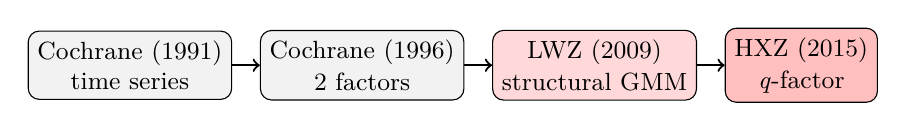
\begin{tikzpicture}[node distance=10pt, every node/.style={font=\small}]
            \node[draw,rounded corners,fill=gray!10] (a) {\shortstack{Cochrane (1991)\\time series}};
            \node[draw,rounded corners,fill=gray!10,right=of a] (b) {\shortstack{Cochrane (1996)\\2 factors}};
            \node[draw,rounded corners,fill=red!15,right=of b] (c) {\shortstack{LWZ (2009)\\structural GMM}};
            \node[draw,rounded corners,fill=red!25,right=of c] (d) {\shortstack{HXZ (2015)\\\textit{q}-factor}};
            \draw[->,thick] (a) -- (b);
            \draw[->,thick] (b) -- (c);
            \draw[->,thick] (c) -- (d);
        \end{tikzpicture}
    \end{center}
\end{frame}

\section{The Investment-Return Relation}

\begin{frame}{From Q-Theory to Expected Returns}
    \textbf{Campbell-Shiller Log-Linearization:}
    
    Take logs and apply Campbell-Shiller approximation to $V_t - D_t = V_t(1 - D_t/V_t)$:
    \begin{equation}\label{equ:campbell shiller}
        \log\left(\phi'\left(\frac{I_t}{K_t}\right)\right) \approx (d_t - k_{t+1}) + \mathrm{E}_t \sum_{j=0}^{\infty} \rho^j \Delta d_{t+1+j} - \mathrm{E}_t \sum_{j=0}^{\infty} \rho^j r_{t+1+j}
    \end{equation}
    
    where:
    \begin{itemize}
        \item $d_t = \log D_t$, $k_t = \log K_t$, $r_t$ is log return
        \item $\rho = 1 - \exp(\overline{d - v}) < 1$ is linearization constant
    \end{itemize}
    
    
    \textbf{Economic Interpretation:}
    \begin{equation*}
        \underbrace{\text{Invest more}}_{\phi' \uparrow} \Leftrightarrow \begin{cases}
            \text{High current profitability} & (d_t - k_{t+1}) \uparrow \\
            \text{Rapid dividend growth} & \sum \rho^j \Delta d_{t+1+j} \uparrow \\
            \text{OR low future returns} & \sum \rho^j r_{t+1+j} \downarrow
        \end{cases}
    \end{equation*}
\end{frame}

\begin{frame}{The Core Prediction: Investment and Returns}
    \textbf{Rearranging (\ref{equ:campbell shiller}):}
    \begin{equation*}
        \mathrm{E}_t \sum_{j=0}^{\infty} \rho^j r_{t+1+j} \approx (d_t - k_{t+1}) + \mathrm{E}_t \sum_{j=0}^{\infty} \rho^j \Delta d_{t+1+j} - \log\left(\phi'\left(\frac{I_t}{K_t}\right)\right)
    \end{equation*}
    
    \textbf{Holding profitability constant:}
    \begin{equation*}
        \frac{\partial \mathrm{E}_t[\sum r_{t+1+j}]}{\partial (I_t/K_t)} < 0
    \end{equation*}
    
    
    \textbf{Key Predictions:}
    \begin{enumerate}
        \item \textbf{Investment effect:} High investment $\rightarrow$ Low future returns
        \begin{itemize}
            \item Firms invest a lot when discount rates (required returns) are low
            \item Investing today reduces marginal productivity of capital tomorrow
        \end{itemize}
        
        \item \textbf{Profitability effect:} High profitability $\rightarrow$ High future returns
        \begin{itemize}
            \item Controlling for investment, profitable firms must offer higher returns
            \item Compensates for risk or reflects temporary mispricing
        \end{itemize}
    \end{enumerate}
\end{frame}

\begin{frame}{Intuition: Why Investment Predicts Returns}
    \textbf{Scenario 1: High Investment Firms}
    \begin{itemize}
        \item Currently investing heavily: $I_t/K_t$ is large
        \item Why? \textbf{Either:}
        \begin{itemize}
            \item Current profitability is high, OR
            \item Expected future profitability is high, OR
            \item Required returns (discount rates) are low
        \end{itemize}
        \item If we control for current and future profitability...
        \item Then high investment must mean low required returns
        \item $\Rightarrow$ Low future stock returns
    \end{itemize}
    
    
    \textbf{Scenario 2: Low Investment Firms}
    \begin{itemize}
        \item Currently investing little: $I_t/K_t$ is small
        \item Could be:
        \begin{itemize}
            \item Profitability is low, OR
            \item Required returns are high (capital is expensive)
        \end{itemize}
        \item Controlling for profitability...
        \item Low investment signals high required returns
        \item $\Rightarrow$ High future stock returns
    \end{itemize}
\end{frame}

\begin{frame}{Intuition: Why Profitability Predicts Returns}
    \textbf{Scenario 1: High Profitability, Low Investment}
    \begin{itemize}
        \item Firm is very profitable: $D_t/K_t$ is large
        \item But investing little: $I_t/K_t$ is small
        \item From Q-theory: $\phi'(I/K) = (D/K) \times (V-D)/D$
        \item Left side is low (low investment), first term on right is high
        \item So $(V-D)/D$ must be low $\rightarrow$ Market values firm cheaply
        \item $\Rightarrow$ High future returns (mean reversion or risk premium)
    \end{itemize}
    
    
    \textbf{Scenario 2: Low Profitability, High Investment}
    \begin{itemize}
        \item Firm has low current profits: $D_t/K_t$ is small
        \item But investing heavily: $I_t/K_t$ is large
        \item Left side is high, first term on right is low
        \item So $(V-D)/D$ must be high $\rightarrow$ Market values firm richly
        \item Expects future improvements, so current returns are low
        \item $\Rightarrow$ Low future returns
    \end{itemize}
    
    \vspace{0.2cm}
    \textbf{Key:} Investment and profitability together pin down expected returns
\end{frame}

\section{Liu, Whited, and Zhang (2009): Making It Empirical}

\begin{frame}{Specifying the Adjustment Cost Function}
    \textbf{Problem:} Q-theory gives general relationship, but need specific form for empirics
    
    \vspace{0.2cm}
    \textbf{\href{https://doi.org/10.1086/649760}{\textcolor{blue}{Liu, Whited, and Zhang (2009)}} Specification:}
    \begin{equation}\label{equ:lwz cost}
        \phi\left(\frac{I_t}{K_t}\right) = \frac{I_t}{K_t} + \frac{a}{2}\left(\frac{I_t}{K_t}\right)^2
    \end{equation}
    
    where $a > 0$ is the adjustment cost parameter
    
    
    \textbf{Properties:}
    \begin{itemize}
        \item \textbf{Purchase cost:} $I_t/K_t$ (just buying the capital)
        \item \textbf{Quadratic adjustment cost:} $\frac{a}{2}(I_t/K_t)^2$ (installation, disruption)
        \item \textbf{Marginal cost:}
        \begin{equation}\label{equ:marginal cost}
            \phi'\left(\frac{I_t}{K_t}\right) = 1 + a\left(\frac{I_t}{K_t}\right)
        \end{equation}
        \item Linear in investment rate: $\phi'$ increases linearly with $I/K$
        \item \textbf{Without adjustment costs:} $a = 0 \Rightarrow \phi' = 1$ (constant)
    \end{itemize}
\end{frame}

\begin{frame}{Computing Marginal Value of Capital}
    \textbf{From Envelope Theorem (\ref{equ:envelope theorem}):}
    \begin{equation*}
        \frac{\partial V_{t+1}}{\partial K_{t+1}} = \alpha \frac{\partial Y_{t+1}}{\partial K_{t+1}} - \frac{\partial \Phi_{t+1}}{\partial K_{t+1}} + (1-\delta) \phi'\left(\frac{I_{t+1}}{K_{t+1}}\right)
    \end{equation*}
    
    \textbf{Step 1: Marginal Product of Capital}
    
    Since $Y_t = Z_t^{1/\alpha} [(1-\alpha)/\omega_t]^{(1-\alpha)/\alpha} K_t$:
    \begin{equation*}
        \frac{\partial Y_{t+1}}{\partial K_{t+1}} = \frac{Y_{t+1}}{K_{t+1}}
    \end{equation*}
    
    \textbf{Step 2: Marginal Effect on Adjustment Costs}
    
    From $\Phi_t = \phi(I_t/K_t) K_t$:
    \begin{equation*}
        \begin{aligned}
            \frac{\partial \Phi_{t+1}}{\partial K_{t+1}} &= \phi\left(\frac{I_{t+1}}{K_{t+1}}\right) - \phi'\left(\frac{I_{t+1}}{K_{t+1}}\right) \frac{I_{t+1}}{K_{t+1}} \\
            &= \left[\frac{I_{t+1}}{K_{t+1}} + \frac{a}{2}\left(\frac{I_{t+1}}{K_{t+1}}\right)^2\right] - \left[1 + a\frac{I_{t+1}}{K_{t+1}}\right] \frac{I_{t+1}}{K_{t+1}} \\
            &= -\frac{a}{2}\left(\frac{I_{t+1}}{K_{t+1}}\right)^2
        \end{aligned}
    \end{equation*}
\end{frame}

\begin{frame}{The Complete Marginal Value Expression}
    \textbf{Combining all terms:}
    \begin{equation}\label{equ:marginal value}
        \boxed{
        \begin{aligned}
            \frac{\partial V_{t+1}}{\partial K_{t+1}} &= \alpha \frac{Y_{t+1}}{K_{t+1}} + \frac{a}{2}\left(\frac{I_{t+1}}{K_{t+1}}\right)^2 + (1-\delta)\left[1 + a\frac{I_{t+1}}{K_{t+1}}\right]
        \end{aligned}
        }
    \end{equation}
    
    
    \textbf{Economic Interpretation - Three Components:}
    \begin{enumerate}
        \item $\alpha Y_{t+1}/K_{t+1}$: Profit per unit of capital
        \begin{itemize}
            \item Direct benefit of more capital: higher output $\rightarrow$ higher profits
        \end{itemize}
        
        \item $\frac{a}{2}(I_{t+1}/K_{t+1})^2$: Adjustment cost saving
        \begin{itemize}
            \item Larger capital base $\rightarrow$ lower adjustment costs per unit
            \item Comes from $-\partial \Phi/\partial K < 0$ (economies of scale)
        \end{itemize}
        
        \item $(1-\delta)[1 + a(I_{t+1}/K_{t+1})]$: Continuation value
        \begin{itemize}
            \item Undepreciated capital survives to next period
            \item Worth its marginal installation cost
        \end{itemize}
    \end{enumerate}
\end{frame}

\begin{frame}{The LWZ Return Formula}
    \textbf{Investment Return Formula:}
    
    From FOC: $\phi'(I_t/K_t) = \mathrm{E}_t[M_{t+1} \partial V_{t+1}/\partial K_{t+1}]$
    
    The gross return on investment is:
    \begin{equation*}
        1 + R_{t+1}^I = \frac{\partial V_{t+1}/\partial K_{t+1}}{\phi'(I_t/K_t)}
    \end{equation*}
    
    \textbf{Substituting our expressions:}
    \begin{equation}\label{equ:lwz return}
        \boxed{
        1 + R_{t+1} = \frac{\alpha \frac{Y_{t+1}}{K_{t+1}} + \frac{a}{2}\left(\frac{I_{t+1}}{K_{t+1}}\right)^2 + (1-\delta)\left[1 + a\frac{I_{t+1}}{K_{t+1}}\right]}{1 + a\frac{I_t}{K_t}}
        }
    \end{equation}
    
    
    \textbf{Key Features:}
    \begin{itemize}
        \item Links realized returns to observable quantities: $Y/K$, $I/K$
        \item No latent variables or unobservable SDFs
        \item Two parameters only: $\alpha$ (capital share), $a$ (adjustment cost)
        \item Can test directly with accounting data
    \end{itemize}
\end{frame}

\begin{frame}{Understanding the LWZ Return Formula}
    \begin{equation*}
        1 + R_{t+1} = \frac{\overbrace{\alpha \frac{Y_{t+1}}{K_{t+1}}}^{\text{Profitability}} + \overbrace{\frac{a}{2}\left(\frac{I_{t+1}}{K_{t+1}}\right)^2 + (1-\delta)\left[1 + a\frac{I_{t+1}}{K_{t+1}}\right]}^{\text{Capital evolution}}}{\underbrace{1 + a\frac{I_t}{K_t}}_{\text{Cost of investing}}}
    \end{equation*}

    \textbf{Numerator (Realized Payoff):}
    \begin{itemize}
        \item High $Y_{t+1}/K_{t+1}$ $\rightarrow$ High return (profitable operations)
        \item High $I_{t+1}/K_{t+1}$ $\rightarrow$ High return (growing, valuable capital)
        \item Low depreciation $\delta$ $\rightarrow$ High return (capital lasts longer)
    \end{itemize}

    \textbf{Denominator (Cost Basis):}
    \begin{itemize}
        \item High $I_t/K_t$ $\rightarrow$ Low return (expensive to invest)
        \item Captures that firms investing heavily face high marginal costs
        \item This cost reduces the return per dollar invested
    \end{itemize}

    \textit{Returns are high when profitability is high and investment was cheap (low $I_t/K_t$)}
\end{frame}

% ---------------------------------------------------------
% New: LWZ empirical implementation details
% (PDF Section 7.1.2, page 213)
% ---------------------------------------------------------
\begin{frame}{LWZ's Empirical Strategy: GMM on Moments}
    \textbf{Why not test the strong-form identity $1+R_{t+1} = 1+R^I_{t+1}$ state-by-state?}
    \begin{itemize}
        \item Such an exact restriction is overwhelmingly rejected by the data.
        \item Driven by measurement error in $Y/K$, $I/K$, and timing mismatches between accounting and market data.
    \end{itemize}

    \vspace{0.2cm}
    \textbf{LWZ's compromise: match moments, not paths.}
    \begin{itemize}
        \item For each test portfolio $i$, define moment conditions:
        \begin{equation*}
            g_i(\theta) = \begin{pmatrix} \mathrm{E}[R_{i,t+1}] - \mathrm{E}[R^I_{i,t+1}(\theta)] \\ \mathrm{Var}(R_{i,t+1}) - \mathrm{Var}(R^I_{i,t+1}(\theta)) \end{pmatrix}
        \end{equation*}
        where $\theta = (\alpha, a)$ are the only structural parameters.
        \item Use \textbf{GMM} to minimize a weighted norm of $\{g_i(\theta)\}$ across portfolios.
    \end{itemize}

    \vspace{0.1cm}
    \textbf{Why this is parsimonious:} Two parameters discipline the cross-section of \textit{both} mean and volatility of returns. No latent factors, no preference parameters.
\end{frame}

\begin{frame}{LWZ's Test Assets and Headline Findings}
    \textbf{Three sets of test portfolios (each capturing an anomaly):}
    \begin{enumerate}
        \item \textbf{Capital investment-sorted:} High-$I/A$ firms have low average returns (\href{https://doi.org/10.1111/j.1540-6261.2004.00709.x}{\textcolor{blue}{Titman, Wei, Xie 2004}}).
        \item \textbf{Earnings-surprise-sorted (SUE):} Post-earnings-announcement drift --- high-SUE firms keep outperforming.
        \item \textbf{Book-to-market-sorted:} The classic value premium.
    \end{enumerate}

    \vspace{0.2cm}
    \textbf{Estimated parameters $(\alpha, a)$ across portfolio types:}
    \small
    \begin{center}
        \begin{tabular}{@{}lcc@{}}
            \toprule
            \textbf{Portfolio sort} & $\alpha$ (capital share) & $a$ (adj.\ cost) \\
            \midrule
            Investment $I/A$ & $0.2$--$0.5$ & \textbf{Low} \\
            Earnings surprise (SUE) & $0.2$--$0.5$ & Intermediate \\
            Book-to-market & $0.2$--$0.5$ & \textbf{Very high} \\
            \bottomrule
        \end{tabular}
    \end{center}

    \vspace{0.1cm}
    \textbf{Reading.}
    \begin{itemize}
        \item Capital share is reasonable and stable across anomalies.
        \item But the adjustment-cost parameter is \textit{not}: it must be much higher for value firms than for investment-sorted firms.
    \end{itemize}
\end{frame}

\begin{frame}{Why Different Anomalies Demand Different $a$}
    \textbf{Mechanics of the LWZ formula (\ref{equ:lwz return}):}
    \begin{equation*}
        1 + R_{t+1} = \frac{\alpha\, Y_{t+1}/K_{t+1} + \frac{a}{2}(I_{t+1}/K_{t+1})^2 + (1-\delta)[1+a(I_{t+1}/K_{t+1})]}{1 + a(I_t/K_t)}
    \end{equation*}

    \vspace{0.1cm}
    \textbf{Investment-sorted (low $a$ suffices):}
    \begin{itemize}
        \item High-investment firms have very high $I_t/K_t$ \textit{today} but much lower $I_{t+1}/K_{t+1}$ tomorrow.
        \item A modestly positive $a$ already pulls down their returns through the denominator. Big $a$ would over-shoot.
    \end{itemize}

    \vspace{0.15cm}
    \textbf{Value-sorted (very high $a$ needed):}
    \begin{itemize}
        \item Growth firms have high investment in \textit{both} periods plus high $Y/K$.
        \item Without large $a$, the formula predicts \textit{high} returns for growth firms --- the opposite of the data.
        \item Forces $a$ to be large enough that the convex cost dominates the profitability term.
    \end{itemize}

    \vspace{0.15cm}
    \begin{block}{The pervasive heterogeneity problem}
        ``Different parameters for different anomalies'' is a chronic disease of $q$-theoretic asset pricing. The cleaner empirical response is the HXZ \textit{q}-factor model, which replaces structural estimation with mimicking-portfolio loadings.
    \end{block}
\end{frame}

\begin{frame}{Beyond Quadratic: Richer Adjustment-Cost Specifications}
    \textbf{The classic quadratic $\phi(I/K) = I/K + (a/2)(I/K)^2$ has known limitations.}

    \vspace{0.15cm}
    \textbf{Three extensions in the literature:}
    \begin{enumerate}
        \item \textbf{Asymmetric costs (\href{https://doi.org/10.1111/j.1540-6261.2004.00709.x}{\textcolor{blue}{Zhang 2005}}):} different $a$ for $I>0$ vs.\ $I<0$ to make disinvestment costlier. Crucial for the value premium (next section).
        \item \textbf{Greater-than-quadratic convexity (\href{https://doi.org/10.1086/520552}{\textcolor{blue}{Merz \& Yashiv, 2007}}):} adjustment costs in \textit{both} capital and labor; super-quadratic curvature. Fits aggregate investment far better than the textbook model.
        \item \textbf{Fixed costs / non-convex costs (\href{https://doi.org/10.2307/2118364}{\textcolor{blue}{Abel \& Eberly, 1994}}):} introduces inaction regions where $I=0$ over a range of $q$.
    \end{enumerate}

    \vspace{0.1cm}
    \textbf{Why this matters for asset pricing:}
    \begin{itemize}
        \item The shape of $\phi(\cdot)$ controls the volatility of $\phi'(\cdot)$, hence the volatility of investment returns.
        \item Different anomalies probe different regions of $\phi(\cdot)$ $\rightarrow$ explains why a single quadratic fails.
    \end{itemize}
\end{frame}

\section{Empirical Implications and Predictions}

\begin{frame}{Testable Predictions from the Model}
    \textbf{Cross-Sectional Predictions:}
    \begin{enumerate}
        \item \textbf{Investment Effect (Negative):}
        \begin{equation*}
            \frac{\partial R_{t+1}}{\partial (I_t/K_t)} < 0
        \end{equation*}
        \begin{itemize}
            \item Firms with high investment rates earn lower future returns
            \item Denominator effect: High $I/K$ means expensive to invest
            \item Consistent with \href{https://doi.org/10.1111/j.1540-6261.2008.01370.x}{\textcolor{blue}{Cooper, Gulen, and Schill (2008)}}
        \end{itemize}
        
        \item \textbf{Profitability Effect (Positive):}
        \begin{equation*}
            \frac{\partial R_{t+1}}{\partial (Y_{t+1}/K_{t+1})} > 0
        \end{equation*}
        \begin{itemize}
            \item Firms with high profitability earn higher returns
            \item Numerator effect: Direct cash flow generation
            \item Consistent with \href{https://doi.org/10.1016/j.jfineco.2013.01.003}{\textcolor{blue}{Novy-Marx (2013)}} 
        \end{itemize}
    \end{enumerate}
\end{frame}

\begin{frame}{Why Investment Predicts Returns: Three Channels}
    \textbf{Channel 1: Diminishing Returns to Capital}
    \begin{itemize}
        \item Investing heavily today $\rightarrow$ More capital tomorrow
        \item More capital $\rightarrow$ Lower marginal productivity (decreasing returns)
        \item Lower productivity $\rightarrow$ Lower future profits
        \item Lower profits $\rightarrow$ Lower returns
    \end{itemize}
    
    \vspace{0.2cm}
    \textbf{Channel 2: Time-Varying Discount Rates}
    \begin{itemize}
        \item Firms invest more when discount rates (required returns) are low
        \item Low current discount rates $\rightarrow$ Low future realized returns
        \item Rational: Optimal to invest when capital is "cheap" (low $r$)
    \end{itemize}
    
    \vspace{0.2cm}
    \textbf{Channel 3: Investment Costs}
    \begin{itemize}
        \item High $I/K$ implies high marginal cost $\phi'$
        \item Return = Benefit / Cost
        \item High cost $\rightarrow$ Lower return per dollar invested
        \item Purely mechanical effect from convex adjustment costs
    \end{itemize}
    
    \vspace{0.2cm}
    \textit{All three channels work in same direction: High investment $\rightarrow$ Low returns}
\end{frame}

\begin{frame}{Why Profitability Predicts Returns}
    \textbf{Direct Mechanism:}
    \begin{itemize}
        \item Return formula has $\alpha (Y/K)$ in numerator
        \item Higher profitability $\rightarrow$ Mechanically higher returns
        \item Reflects that profitable firms generate more cash flow
    \end{itemize}
    
    
    \textbf{But Why Does Profitability Persist?}
    \begin{enumerate}
        \item \textbf{Mean Reversion is Slow:}
        \begin{itemize}
            \item Profitable firms stay profitable for years
            \item Barriers to entry, competitive advantages
            \item Adjustment costs prevent immediate convergence
        \end{itemize}
        
        \item \textbf{Growth Options:}
        \begin{itemize}
            \item Profitable firms can expand into new markets
            \item Reinvest profits at high marginal returns
            \item Creates persistence in profitability
        \end{itemize}
        
        \item \textbf{Risk-Based Story:}
        \begin{itemize}
            \item Profitability may proxy for exposure to systematic risk
            \item Profitable firms = low distress risk
            \item Or profitable firms carry different factor exposures
        \end{itemize}
    \end{enumerate}
\end{frame}


\begin{frame}{Relation to Fama-French Factors}
    \textbf{\href{https://doi.org/10.1016/j.jfineco.2014.10.010}{\textcolor{blue}{Fama-French 5-Factor Model (2015)}}:} 2014.10
    \begin{equation*}
    \begin{aligned}
        R_i - R_f &= \alpha + \beta_{MKT}(R_M - R_f) + \beta_{SMB}SMB + \beta_{HML}HML \\ 
        &+ \beta_{RMW}RMW + \beta_{CMA}CMA
    \end{aligned}
    \end{equation*}
    
    \textbf{Production-Based Interpretation:}
    \begin{itemize}
        \item \textbf{RMW (Robust Minus Weak):} Profitability factor
        \begin{itemize}
            \item Long high operating profitability, short low profitability
            \item Directly related to $Y/K$ in production model
        \end{itemize}
        
        \item \textbf{CMA (Conservative Minus Aggressive):} Investment factor
        \begin{itemize}
            \item Long low investment firms, short high investment firms
            \item Directly related to $I/K$ in production model
        \end{itemize}
    \end{itemize}
\end{frame}


% =========================================================
% New section: explaining firms' betas via production
% (PDF Section 7.1.3, Zhang 2005)
% =========================================================
\section{Explaining Firms' Betas: Zhang (2005)}

\begin{frame}{From Pricing to Betas: A Different Question}
    \textbf{So far:} We have priced the cross-section using investment + profitability \textit{characteristics}.

    \vspace{0.2cm}
    \textbf{Now ask:} Why do \textit{value} firms \textbf{covary more strongly with the SDF} than \textit{growth} firms?
    \begin{itemize}
        \item This is the original Fama-French (1992) value premium puzzle.
        \item Empirically: high B/M (value) firms earn higher average returns and have higher betas in some periods.
        \item The challenge: \textbf{generate} the value premium endogenously from a production model with an exogenous SDF.
    \end{itemize}

    \vspace{0.2cm}
    \textbf{\href{https://doi.org/10.1111/j.1540-6261.2004.00709.x}{\textcolor{blue}{Zhang (2005, JF)}}: ``The value premium''}
    \begin{itemize}
        \item Take a heteroskedastic single-factor SDF as given (rules out behavioral channels).
        \item Add \textbf{asymmetric} adjustment costs: it is more costly to disinvest than to invest.
        \item Show that this asymmetry generates a sizable value premium endogenously.
    \end{itemize}
\end{frame}

\begin{frame}{Zhang (2005): The SDF and Productivity}
    \textbf{Heteroskedastic single-factor SDF (in logs):}
    \begin{equation}\label{equ:zhang sdf}
        m_{t+1} = \log\beta - \gamma_t (x_{t+1} - x_t)
    \end{equation}
    \begin{equation}\label{equ:zhang gamma}
        \gamma_t = \gamma_0 + \gamma_1 (x_t - \bar{x}), \qquad \gamma_1 < 0
    \end{equation}
    where $x_t$ is aggregate (log) productivity following an AR(1).

    \textbf{Read.} The price of risk $\gamma_t$ rises in bad times ($x_t$ low) --- countercyclical risk aversion baked in.

    \vspace{0.2cm}
    \textbf{Idiosyncratic productivity for firm $j$:}
    \begin{itemize}
        \item $z_{jt}$ follows AR(1) with common persistence.
        \item \textbf{Value} firms: low current $z_{jt}$ $\rightarrow$ low productivity, low investment, low profits.
        \item \textbf{Growth} firms: high current $z_{jt}$ $\rightarrow$ high productivity, high investment.
    \end{itemize}

    \vspace{0.2cm}
    \textbf{Conditional CAPM holds by construction}, but the model still generates a sizable \textit{unconditional} value premium.
\end{frame}

\begin{frame}{The Asymmetric Adjustment Cost}
    \textbf{Quadratic but kinked at $I=0$:}
    \begin{equation}\label{equ:zhang cost}
        \phi_{jt} = \frac{I_{jt}}{K_{jt}} + \frac{a_{jt}}{2}\left(\frac{I_{jt}}{K_{jt}}\right)^2,
        \qquad a_{jt} = \begin{cases} a^+ & \text{if } I_{jt} > 0 \\ a^- & \text{if } I_{jt} < 0 \end{cases}
    \end{equation}
    with the central restriction
    \begin{equation*}
        \boxed{a^- > a^+}
    \end{equation*}

    \vspace{0.1cm}
    \textbf{Why this asymmetry is realistic.}
    \begin{itemize}
        \item Used capital markets are illiquid; reselling installed capital incurs large discounts.
        \item Layoff and reorganization costs are concentrated on the disinvestment side.
        \item Specific human capital, learning-by-doing, and contract rigidities all create downward inflexibility.
    \end{itemize}

    \vspace{0.1cm}
    \textbf{Empirical micro-evidence:} \href{https://doi.org/10.1086/250002}{\textcolor{blue}{Caballero, Engel, Haltiwanger (1995)}}; \href{https://www.jstor.org/stable/2233834}{\textcolor{blue}{Cooper-Haltiwanger (2006)}}.
\end{frame}

\begin{frame}{The Mechanism: Who Bears the Bad-Times Risk?}
    \textbf{Calibration outcome.}
    \begin{itemize}
        \item In good times: both value and growth firms invest, but \textbf{growth invests more} $\rightarrow$ pays the high $a^+$ at the margin.
        \item In bad times: growth still invests modestly, but \textbf{value disinvests} $\rightarrow$ pays the much higher $a^-$ at the margin.
    \end{itemize}

    \vspace{0.2cm}
    \begin{center}
        \small
        \begin{tabular}{@{}lcc@{}}
            \toprule
            & \textbf{Good times} & \textbf{Bad times} \\
            \midrule
            \textbf{Growth} (high $z_j$) & high $I/K$, high $a^+$ cost & moderate $I/K$, $a^+$ cost \\
            \textbf{Value} (low $z_j$) & moderate $I/K$, $a^+$ cost & disinvest, \textbf{high $a^-$ cost} \\
            \bottomrule
        \end{tabular}
    \end{center}

    \vspace{0.2cm}
    \textbf{Implication for risk:}
    \begin{itemize}
        \item Firms with \textbf{low} adjustment costs at the margin can smooth dividends $\rightarrow$ less risky.
        \item Firms with \textbf{high} adjustment costs cannot smooth $\rightarrow$ more risky.
        \item \textbf{Growth} firms are riskier in \textit{good} times; \textbf{value} firms are riskier in \textit{bad} times.
    \end{itemize}
\end{frame}

\begin{frame}{Why an Unconditional Value Premium Emerges}
    \textbf{Combining the asymmetric exposure with the heteroskedastic SDF:}
    \begin{itemize}
        \item Value firms are risky exactly when the price of risk $\gamma_t$ is \textit{high} (bad times).
        \item Growth firms are risky when the price of risk is \textit{low} (good times).
        \item Unconditional expected return: $\mathrm{E}[R_j] - R_f \approx -\mathrm{Cov}(M_{t+1}, R_{j,t+1})$.
        \item Same $\beta$ is rewarded more if the covariance lands in high-$\gamma_t$ states.
    \end{itemize}

    \vspace{0.2cm}
    \begin{equation*}
        \underbrace{\mathrm{E}[R^V] - \mathrm{E}[R^G]}_{\text{Value premium}} > 0
        \;\;\Leftarrow\;\;
        \underbrace{\text{Value risk in bad times}}_{\text{high price of risk}}
        \;>\;
        \underbrace{\text{Growth risk in good times}}_{\text{low price of risk}}
    \end{equation*}

    \vspace{0.1cm}
    \begin{block}{Take-away}
        Production technology + asymmetric adjustment costs is enough to \textbf{endogenize} a value premium from an exogenous SDF, without invoking behavioral mispricing.
    \end{block}
\end{frame}

\begin{frame}{Limitations and Modern Extensions}
    \textbf{What Zhang (2005) cannot deliver:}
    \begin{itemize}
        \item Imposes the \textbf{conditional CAPM} by construction $\rightarrow$ only \textit{small} unconditional CAPM-alpha can arise.
        \item Cannot match the post-1990s evidence that value firms have \textbf{lower} CAPM betas than growth firms.
        \item Silent on momentum and other non-value anomalies.
    \end{itemize}

    \vspace{0.2cm}
    \textbf{Generalizations (alternative SDFs that deviate further from the CAPM):}
    \begin{itemize}
        \item \href{https://doi.org/10.1093/rfs/hht067}{\textcolor{blue}{Bazdresch, Belo, Lin (2014)}}: shocks to adjustment costs.
        \item \href{https://doi.org/10.1111/jofi.12080}{\textcolor{blue}{Kogan and Papanikolaou (2014)}}: investment-specific technology shocks lower the price of investment goods; growth options provide insurance.
        \item \href{https://doi.org/10.1093/rfs/hhx135}{\textcolor{blue}{McQuade (2018)}}: positive volatility shocks raise marginal utility; growth firms hedge them.
    \end{itemize}

    \vspace{0.1cm}
    \textbf{Common thread.} Move beyond a CAPM-style SDF to capture insurance value of growth options or aversion to specific shock types.
\end{frame}

% =========================================================
% New section: the FF5 vs Q-factor showdown
% =========================================================
\section{The Showdown: FF5 vs. \textit{q}-Factor}

% ---------------------------------------------------------
% Prologue: narrative tee-up
% ---------------------------------------------------------
\begin{frame}{Prologue: A Decade-Long Drama in Asset Pricing}
	The FF5--Q4 showdown is the public face of a fifteen-year contest that played out behind the scenes at \textit{Journal of Finance}.
	\begin{itemize}
		\item \textbf{2009}: ``A Better Three-Factor Model'' is \textit{accepted} at JF for April 2010 --- then \textit{pulled} at the last moment.
		\item \textbf{2010--2011}: revised version held for a year, then rejected.
		\item \textbf{2012}: Zhang rebuilds his team with Hou and Xue; the model finally appears in RFS 2015.
		\item \textbf{2015}: in the same window, FF publish FF5 with two of the same variables but a different motivation.
	\end{itemize}
	\begin{block}{Why we tell this story}
		Asset pricing models are competing narratives about the same data. \textit{Which} model became dominant and \textit{why} is as important as the regressions.
	\end{block}
	\vspace{2pt}
	{\tiny\textit{Source: Zhang (2016, Tsinghua Financial Review); HXZ (2015) acknowledgements; Harvey (2011) editor report.}}
\end{frame}

% ---------------------------------------------------------
% Q-factor lineage: refined with full dates
% ---------------------------------------------------------
\begin{frame}[allowframebreaks]{The Lu Zhang Program: From ``Neoclassical Factors'' (2007) to HXZ (2015)}
	\small
	A single research program, eight years, six title changes:
	\vspace{4pt}
	\begin{enumerate}
		\item \textbf{1991} \quad \href{https://doi.org/10.1111/j.1540-6261.1991.tb03750.x}{\textcolor{blue}{Cochrane (JF)}} ``Production-based asset pricing'' --- financial returns equal investment returns in equilibrium.
		\item \textbf{2007} \quad NBER WP 13282 ``Neoclassical Factors'' (Liu--Whited--Zhang). First attempt to price returns with the investment FOC.
		\item \textbf{Jan 2009} \quad ``An Equilibrium Three-Factor Model'' (Chen--Zhang).
		\item \textbf{Apr 2009} \quad ``Production-Based Factors'' (Chen--Zhang).
		\item \textbf{End 2009} \quad ``\href{https://static1.squarespace.com/static/5e6033a4ea02d801f37e15bb/t/5f61583e88f43b7d5b7196b5/1600215105801/Chen_Zhang_JF.pdf}{\textcolor{red}{A Better Three-Factor Model That Explains More Anomalies}}'' --- \textit{accepted at JF Vol.\ 65(2), April 2010}. Title imposed by a senior referee (reportedly Sheridan Titman).
		\item \textbf{2010} \quad Paper \textit{withdrawn} after Robert Novy-Marx flags a timing error; revision resubmitted in April 2010.
		\item \textbf{Apr 2011} \quad Revised version \textit{rejected} after a year-long review.
		\item \textbf{2011} \quad SSRN WP ``An Alternative Three-Factor Model'' (\href{https://doi.org/10.2139/ssrn.1418117}{\textcolor{blue}{Chen, \textit{Novy-Marx}, Zhang}}).
		\item \textbf{2012} \quad NBER WP ``Digesting Anomalies'' (Hou--Xue--Zhang). New team, four-factor form (adds Size).
		\item \textbf{2015} \quad Published as \href{https://doi.org/10.1093/rfs/hhu068}{\textcolor{blue}{HXZ (2015, RFS)}}, editor's choice and lead article.
	\end{enumerate}
\end{frame}

% ---------------------------------------------------------
% The 2009 JF paper that almost was
% ---------------------------------------------------------
\begin{frame}{The 2009 JF Paper That Almost Was}
	The version slated for JF April 2010 used the working title ``\textit{Production-Based Factors}.'' A senior referee insisted on a more confrontational title:
	\vspace{6pt}
	\begin{center}
		\large \textbf{``A Better Three-Factor Model That Explains More Anomalies''}
	\end{center}
	\vspace{4pt}
	Zhang has since written that he opposed the title but was overruled. The framing was a direct shot at \href{https://doi.org/10.1016/0304-405X(93)90023-5}{\textcolor{blue}{Fama-French (1993)}}.
	\vspace{6pt}
	\begin{block}{Why titles matter in asset pricing}
		``Better'' and ``more'' implicitly demote FF3 from \textit{the} model to \textit{a} model. Had this paper appeared in JF in April 2010, the empirical asset pricing reading list of 2010--2015 would look very different.
	\end{block}
	\vspace{4pt}
	\tiny\textit{Quotation reconstructed from Zhang (2016, ``Factors War,'' Tsinghua Financial Review). The identity of the senior referee has never been formally confirmed.}
\end{frame}

% ---------------------------------------------------------
% Anatomy of the timing error -- technical detail
% ---------------------------------------------------------
\begin{frame}[allowframebreaks]{Anatomy of the Timing Error}
	\textbf{What broke?} The profitability factor in the JF version was built monthly with a blanket \textbf{4-month lag} from fiscal quarter end:
	\[
		\text{ROA}_t \;=\; \frac{\text{IB}_{q}}{\text{Total Assets}_{q-1}}, \qquad t \;=\; (\text{fiscal quarter end of } q) + 4\text{ months}.
	\]
	The implicit assumption was that, by 4 months after fiscal quarter end, every firm's earnings are already public. \textbf{Not quite.}
	\vspace{6pt}
	\textbf{Why a 4-month lag is not always safe} (SEC filing rules):
	\begin{itemize}
		\item 10-Q (quarterly): due within 40 or 45 days of fiscal quarter end.
		\item 10-K (annual): due within 75--90 days of fiscal year end.
		\item \textbf{NT (Non-Timely) filings}: an extra 5 days for 10-Qs, 15 days for 10-Ks --- and in practice often \textit{much} longer.
	\end{itemize}

    \framebreak
	Audit Analytics (2014) documented \textbf{201 NT filings} across NYSE/AMEX/NASDAQ between 2011 and 2013, with a non-trivial tail of firms taking $>$90 days post-NT filing to actually disclose. A blanket 4-month lag from fiscal quarter end \textbf{could include earnings the market had not yet seen} --- look-ahead bias.
	
	\textbf{What Novy-Marx spotted}\quad For a fraction of firms in each cross-section, the factor was using earnings that were not yet public at portfolio formation, biasing the profitability sort.
	\vspace{6pt}
	\textbf{The fix in HXZ (2015):}
	\begin{enumerate}
		\item Switch the profitability factor from \textbf{ROA} (assets in the denominator) to \textbf{ROE} (book equity in the denominator). Both keep ``income before extraordinary items'' (Compustat \texttt{IBQ}) in the numerator.
		\item Stop using a blanket 4-month lag for earnings. Use the \textbf{actual \texttt{RDQ}} field (Compustat \textit{quarterly earnings announcement date}): a firm enters the sort \textit{only after} its earnings have been publicly announced.
		\item Require the fiscal quarter end of the announced earnings to lie within 6 months prior to portfolio formation (filters stale data).
	\end{enumerate}
	\vspace{4pt}
	\begin{block}{The lesson, and the credit}
		The economic content never changed. What changed was the data plumbing: \textbf{point-in-time} earnings instead of a calendar-based lag. The HXZ (2015) acknowledgements preserve the credit to Novy-Marx --- ``We are extremely grateful to Robert Novy-Marx for identifying a timing error in the empirical analysis of the previous work.''
	\end{block}
\end{frame}

% ---------------------------------------------------------
% Four years of limbo + FF5 coincidence
% ---------------------------------------------------------
\begin{frame}[allowframebreaks]{Four Years of Limbo, and a Suspicious FF5 Coincidence}
	\textbf{April 2010}: the corrected version returns to JF.
	\vspace{2pt}
	\textbf{April 2011}: rejected after a \textit{full year} of review. By Zhang's account, this was ``the darkest time of my career.''
	\vspace{4pt}
	\begin{itemize}
		\item Harvey's 2010 JF editor report claims no paper was in review more than 187 days. The Chen-Zhang revision's actual timeline does not square cleanly with that report.
		\item The team rebuilds. Hou and Xue join; Size is added as a fourth factor; the 2012 NBER WP ``Digesting Anomalies'' is born.
	\end{itemize}
	\framebreak
	\textbf{The 2014--2015 timeline that raises eyebrows:}
	\begin{center}
		\footnotesize
		\begin{tabular}{@{}lll@{}}
			\toprule
			Date & HXZ & FF5 \\
			\midrule
			Aug 2014 & accepted at \textit{RFS} & --- \\
			Sep 2014 & --- & accepted at \textit{JFE} \\
			Mar 2015 & published (lead article) & --- \\
			Apr 2015 & --- & published \\
			\bottomrule
		\end{tabular}
	\end{center}
	\vspace{4pt}
	\begin{block}{The opportunity cost of a four-year delay}
		Had HXZ appeared in JF April 2010 as planned, it would have predated FF5 by five years and the textbook narrative would arguably read ``q-factor first.'' Instead, FF5 inherited the throne of FF3 essentially uncontested.
	\end{block}
\end{frame}

% ---------------------------------------------------------
% HXZ theory frame
% ---------------------------------------------------------
\begin{frame}{HXZ (2015): The Investment FOC at Work}
	\textbf{Two-period economy, quadratic adjustment costs.} Firm $i$'s investment FOC delivers $1 + a\,I_{i0}/A_{i0} = E_0[M_1\,\Pi_{i1}]$, and under constant returns to scale the stock return collapses to
	\[
		r^S_{i,1} \;=\; \frac{\Pi_{i,1}}{1 + a\, I_{i,0}/A_{i,0}} \quad\Longrightarrow\quad E_0[r^S_{i,1}] \;=\; \frac{E_0[\Pi_{i,1}]}{1 + a\,I_{i,0}/A_{i,0}}.
	\]
	\textbf{Two cross-sectional predictions} (holding the other variable fixed):
	\begin{itemize}
		\item \textbf{High $I/A \Rightarrow$ low expected return} (investment channel).
		\item \textbf{High expected profitability $\Rightarrow$ high expected return} (profitability channel).
	\end{itemize}
	\begin{block}{Why this matters for the showdown with FF5}
		Both predictions follow from \textit{firm} optimization, not from a discount factor specification. HXZ's factors are projections of the optimal investment rule onto observable characteristics, not patches on FF3 motivated by accounting identities.
	\end{block}
\end{frame}

% ---------------------------------------------------------
% Constructing the four q-factors (refined with RDQ emphasis)
% ---------------------------------------------------------
\begin{frame}[allowframebreaks]{Constructing the Four \textit{q}-Factors: The RDQ Fix in Detail}
	\small
	\textbf{Variables.}
	\begin{itemize}
		\item \textbf{ME}: price $\times$ shares outstanding (CRSP), end of June.
		\item \textbf{I/A}: $\Delta$ total assets $/$ total assets$_{-1}$ (Compustat annual \texttt{AT}). Annual.
		\item \textbf{ROE}: \texttt{IBQ}$_q$ $/$ book equity$_{q-1}$ (Compustat quarterly). \textit{Monthly}, point-in-time.
	\end{itemize}
	\vspace{2pt}
	\textbf{Sample.} CRSP common stocks, NYSE/AMEX/NASDAQ. Excludes financials and firms with negative book equity. \textbf{1972/01--2012/12}; start date dictated by quarterly earnings announcement (\texttt{RDQ}) coverage.
	\vspace{4pt}
	\textbf{Triple 2$\times$3$\times$3 sort.}
	\begin{itemize}
		\item End of June year $t$: median NYSE \textit{Size} $\rightarrow$ 2 groups.
		\item End of June year $t$: NYSE 30/40/30 breakpoints of \textit{I/A} for the fiscal year ending in $t-1$ $\rightarrow$ 3 groups.
		\item Each \textit{month} $m$: NYSE 30/40/30 breakpoints of \textit{ROE} computed with the most recent earnings announcement $\rightarrow$ 3 groups.
	\end{itemize}
	Intersections give 18 portfolios.
	\framebreak
	\textbf{The point-in-time discipline} (this is the bug fix from 2010):
	\begin{itemize}
		\item Earnings data are used \textit{only} from months \textbf{immediately after} the public quarterly announcement date \texttt{RDQ}. Example: earnings for Q4 of year $t-1$ announced 5 March year $t$ $\Rightarrow$ used to form portfolios at the \textit{beginning of April} year $t$.
		\item The fiscal quarter end of the announced earnings must lie within 6 months prior to portfolio formation. This safeguards against stale earnings.
		\item Note the asymmetry: for \textit{non-earnings} quarterly variables (where there is no \texttt{RDQ}), HXZ still use a 4-month lag --- the very lag that broke the JF version when applied to earnings.
	\end{itemize}
	\vspace{4pt}
	\textbf{Factor returns} (averages across the 18 corner portfolios):
	\begin{itemize}
		\item $r_{\text{ME}}$: small avg.\ $-$ big avg.\ (9 small $-$ 9 big).
		\item $r_{\text{I/A}}$: low-investment avg.\ $-$ high-investment avg.\ (6 $-$ 6).
		\item $r_{\text{ROE}}$: high-ROE avg.\ $-$ low-ROE avg.\ (6 $-$ 6).
	\end{itemize}
	\vspace{2pt}
	\textbf{Rebalancing.} Size and I/A portfolios annually (end of June). ROE portfolios \textbf{monthly}. \textit{Monthly} ROE rebalancing is precisely what creates the timing-error danger zone --- and what makes the \texttt{RDQ}-based safeguard essential.
\end{frame}

% ---------------------------------------------------------
% HXZ empirical headlines
% ---------------------------------------------------------
\begin{frame}{HXZ Empirical Headlines: 80 Anomalies on Trial}
	\small
	\textbf{The universe} (1972--2012). 80 candidate predictors. With NYSE breakpoints and value-weighted returns, \textbf{about half are insignificant} in the broad cross-section --- including 12 of 13 trading-frictions anomalies.
	\vspace{4pt}
	\textbf{Among the 35 anomalies that survive screening:}
	\begin{center}
		\footnotesize
		\begin{tabular}{lccc}
			\toprule
			Model & $\overline{|\alpha_{H{-}L}|}$ & \#\{|t|$>$1.96\} & GRS rej.\ \\
			\midrule
			FF3 & 0.55\% & 27 & 28 \\
			Carhart 4 & 0.33\% & 19 & 24 \\
			\textbf{Q4 (HXZ)} & \textbf{0.20\%} & \textbf{5} & \textbf{20} \\
			\bottomrule
		\end{tabular}
	\end{center}
	\vspace{2pt}
	\textbf{Where Q4 wins big.}\ Momentum (via ROE loadings), profitability (via ROE), net stock issues / accruals / composite issuance (via I/A).
	\vspace{2pt}
	\textbf{Where Q4 underperforms.}\ Operating accruals (OA) and R\&D-to-market: GAAP expenses R\&D, mechanically depressing ROE for innovative firms.
\end{frame}

% ---------------------------------------------------------
% FF5 motivation from DDM (refined with full equations)
% ---------------------------------------------------------
\begin{frame}[allowframebreaks]{How FF5 Defends Itself: The DDM Detour}
	\href{https://doi.org/10.1016/j.jfineco.2014.10.010}{\textcolor{blue}{Fama and French (2015)}} motivate RMW and CMA from the dividend discount model. Start from
	\begin{equation}\label{equ:市值等于未来股利贴现-c}
		m_{t}\;=\;\sum_{\tau=1}^{\infty} \mathrm{E}\!\left(d_{t+\tau}\right) /(1+r)^{\tau},
	\end{equation}
	and use \href{http://www.jstor.org/stable/2351143}{\textcolor{blue}{Miller--Modigliani (1961)}} with clean-surplus accounting ($d = Y - dB$):
	\begin{equation}\label{equ:股利换成盈利减去投资-c}
		M_{t}\;=\;\sum_{\tau=1}^{\infty} \mathrm{E}\!\left(Y_{t+\tau}-dB_{t+\tau}\right) /(1+r)^{\tau}.
	\end{equation}
	Dividing by book equity:
	\begin{equation}\label{equ:市值账面比-c}
		\frac{M_{t}}{B_{t}}\;=\;\frac{\sum_{\tau=1}^{\infty} \mathrm{E}(Y_{t+\tau}-dB_{t+\tau}) /(1+r)^{\tau}}{B_{t}}.
	\end{equation}
	\vspace{2pt}
	\textbf{Three statements about expected returns} from (\ref{equ:市值账面比-c}):
	\begin{enumerate}
		\item Lower $M_t/B_t$ (higher B/M), \textit{holding $E[Y]$ and $E[dB]$ fixed}, $\Rightarrow$ higher $r$. \quad $\Rightarrow$ HML.
		\item Higher expected earnings $E[Y]$, \textit{holding M/B and $E[dB]$ fixed}, $\Rightarrow$ higher $r$. \quad $\Rightarrow$ RMW.
		\item Higher expected investment $E[dB]$, \textit{holding M/B and $E[Y]$ fixed}, $\Rightarrow$ \textbf{lower} $r$. \quad $\Rightarrow$ CMA.
	\end{enumerate}
	\vspace{4pt}
	\begin{block}{Why HXZ call this a defense, not a derivation}
		Equation (\ref{equ:市值账面比-c}) is an \textbf{accounting identity}; it has no structural content beyond the DDM itself. The economic mechanism (\textit{why} expected investment should relate to discount rates) is read off ex post. HXZ's complaint: ``you reached the same variables but skipped the production model.''
	\end{block}
	\framebreak
	\textbf{FF5 variable definitions:}
	\begin{itemize}
		\item \textbf{Operating profitability (OP)} for the June-of-$t$ sort: from $t-1$ annual financials, $(\text{Revenues} - \text{COGS} - \text{SG\&A} - \text{Interest expense})\,/\,\text{Book equity}$. \textbf{Annual update.}
		\item \textbf{Investment (Inv)}: $\Delta$Total Assets from $t-2$ to $t-1$, divided by Total Assets$_{t-2}$.
	\end{itemize}
	\vspace{4pt}
	\begin{block}{Note from FF (2015) and the first big difference from HXZ}
		FF (2015) note that ``the investment variable is the expected growth of \textit{book equity}, not assets,'' but use asset growth as a proxy (consistent with HXZ). \textbf{The bigger gap is timing}: FF5 updates profitability \textit{annually} from year $t-1$ financials, whereas HXZ updates ROE \textit{monthly} as each new \texttt{RDQ} arrives. That single design choice is the main reason the Q4 absorbs momentum and FF5 does not.
	\end{block}
\end{frame}

% ---------------------------------------------------------
% FF5 factor construction: three sort choices
% ---------------------------------------------------------
\begin{frame}{FF5 Factor Construction: Three Sort Choices}
	\small
	Fama--French (2015) actually consider \textbf{three} ways to build the factors, to test sensitivity to portfolio design:
	\vspace{4pt}
	\begin{enumerate}
		\item \textbf{2$\times$3 sorts} (FF93 tradition): independent sort on Size and \textit{one} of $\{$B/M, OP, Inv$\}$, NYSE median for Size, NYSE 30/70 for the other variable. 6 portfolios per sort. Drops the middle 40\% of the second variable.
		\item \textbf{2$\times$2 sorts}: NYSE medians for both variables; includes the middle of the distribution. Better diversified, smaller premium spreads, similar Sharpe ratios.
		\item \textbf{2$\times$2$\times$2$\times$2 sorts}: jointly control for Size, B/M, OP, Inv. 16 portfolios. ``Cleanest'' marginal premiums but with messy correlations (HML--RMW correlation jumps to 0.63!).
	\end{enumerate}
	\vspace{4pt}
	\textbf{Headline factor premiums in 1963--2013 (2$\times$3 sorts):}
	\begin{center}
		\begin{tabular}{lcccc}
			\toprule
			& SMB & HML & RMW & CMA \\
			\midrule
			Mean (\%/mo) & 0.29 & 0.37 & 0.25 & 0.33 \\
			$t$ & 2.31 & 3.20 & 2.92 & 4.07 \\
			\bottomrule
		\end{tabular}
	\end{center}
	\vspace{2pt}
	All four clear the standard $|t|>2$ hurdle; CMA and HML clear the \href{https://doi.org/10.1093/rfs/hhv059}{\textcolor{blue}{Harvey--Liu--Zhu (2016)}} $|t|>3$ multiple-testing hurdle outright.
\end{frame}

% ---------------------------------------------------------
% FF's own admission: HML is redundant
% ---------------------------------------------------------
\begin{frame}[allowframebreaks]{Fama--French's Own Admission: HML Is Redundant}
	A striking result \textit{inside} Fama--French (2015), Table 6. Regress each factor on the other four:
	\vspace{4pt}
	\begin{center}
		\small
		\begin{tabular}{lcccccc}
			\toprule
			\textbf{LHS} & $\alpha$ & $t(\alpha)$ & $b_{\text{Mkt}}$ & $b_{\text{HML}}$ & $b_{\text{RMW}}$ & $b_{\text{CMA}}$ \\
			\midrule
			$R_M - R_F$ & 0.82 & 4.94 & --- & 0.03 & $-$0.40 & $-$0.91 \\
			SMB         & 0.39 & 3.23 & 0.13 & 0.05 & $-$0.48 & $-$0.17 \\
			\textbf{HML} & $\mathbf{-0.04}$ & $\mathbf{-0.47}$ & 0.01 & --- & 0.23 & \textbf{1.04} \\
			RMW         & 0.43 & 5.45 & $-$0.09 & 0.20 & --- & $-$0.44 \\
			CMA         & 0.28 & 5.03 & $-$0.10 & 0.45 & $-$0.21 & --- \\
			\bottomrule
		\end{tabular}
	\end{center}
	\vspace{4pt}
	\textbf{Read the HML row.} $t(\alpha) = -0.47$. HML's average return is \textit{fully} absorbed by Mkt, SMB, RMW, and especially CMA (slope $1.04$, $t = 23.0$ in the underlying regression).
	\framebreak
	\begin{block}{Fama and French's own conclusion}
		``Adding HML does not improve the mean-variance-efficient tangency portfolio produced by combining the riskfree asset, the market portfolio, SMB, RMW, and CMA.'' \\[2pt]
		\textit{In FF5's own data, HML is redundant.} HXZ had been making this argument since 2010 with I/A and ROE; FF5 confirms it using CMA and RMW.
	\end{block}
\end{frame}

% ---------------------------------------------------------
% Head-to-head comparison
% ---------------------------------------------------------
\begin{frame}{Head-to-Head: FF5 vs.\ Q4}
	\scriptsize
	\begin{tabular}{@{}lp{0.36\linewidth}p{0.36\linewidth}@{}}
		\toprule
		& \textbf{FF5} (\href{https://doi.org/10.1016/j.jfineco.2014.10.010}{\textcolor{blue}{Fama--French 2015}}) & \textbf{Q4} (\href{https://doi.org/10.1093/rfs/hhu068}{\textcolor{blue}{Hou--Xue--Zhang 2015}}) \\
		\midrule
		Factors & MKT, SMB, HML, RMW, CMA & MKT, ME, I/A, ROE \\
		\addlinespace
		Theoretical foundation & DDM accounting identity (\textit{ex post}) & Investment Euler equation (\textit{ex ante}) \\
		\addlinespace
		Profitability proxy & Operating profitability, \textbf{annual} update & ROE, \textbf{monthly} update on \texttt{RDQ} \\
		\addlinespace
		Investment proxy & $\Delta$Assets/Assets, annual & $\Delta$Assets/Assets, annual \\
		\addlinespace
		Sort design & 2$\times$3 (also 2$\times$2 and 2$\times$2$\times$2$\times$2 reported) & 2$\times$3$\times$3 triple sort \\
		\addlinespace
		Role of HML & ``Core'' factor, but redundant in FF5's own spanning test & Absent (not in the model) \\
		\addlinespace
		Anomaly explanation & Strong on value, profitability, investment; \textbf{weak on momentum} (need FF6) & Strong on momentum (via ROE), profitability, investment; weak on accruals, R\&D \\
		\bottomrule
	\end{tabular}
	\vspace{4pt}
	\begin{center}
		\footnotesize \textit{Same DNA, different parents. The disagreement is over timing convention and theoretical origin --- not which variables matter.}
	\end{center}
\end{frame}

% ---------------------------------------------------------
% Hou-Mo-Xue-Zhang (2019) — the formal horse race
% ---------------------------------------------------------
\begin{frame}{The Formal Horse Race: \href{https://doi.org/10.1093/rof/rfy032}{\textcolor{blue}{Hou--Mo--Xue--Zhang (2019)}} ``Which Factors?''}
	HMXZ run spanning-regression tests between Q4, FF5, FF6, and Stambaugh--Yuan (2017) on 150 anomalies. The paper won the 2019 \textit{RoF} Spangle IQAM Best Paper Prize.
	\vspace{4pt}
	\textbf{Three sharp results:}
	\begin{enumerate}
		\item \textbf{HML and CMA are redundant} once I/A and ROE are included; their alphas vs.\ Q4 are tiny and insignificant.
		\item \textbf{Q4 spans FF5}: Q4 attains the FF5 squared Sharpe ratio with strictly fewer factors.
		\item \textbf{FF5 does \textit{not} span Q4}: ROE cannot be replicated as a linear combination of FF5 factors --- its alpha against FF5 is large and significant.
	\end{enumerate}
	\begin{block}{Implication}
		On squared Sharpe ratio and spanning, the \textit{q}-factor model dominates FF5. \textbf{This is the core ammunition of the Lu Zhang camp in the Factor War} --- and reads, to sympathetic eyes, as a quiet rebuttal to whatever process delayed the original paper from 2010 to 2015.
	\end{block}
\end{frame}

% ---------------------------------------------------------
% q5 extension — with full technical detail
% ---------------------------------------------------------
\begin{frame}[allowframebreaks]{The $q^5$ Extension: Adding Expected Growth (\href{https://doi.org/10.1093/rof/rfaa004}{\textcolor{blue}{HMXZ 2021}})}
	\textbf{Motivation.} The Q4 leaves residual alphas on anomalies driven by \textit{future} investment growth (R\&D-to-market, accruals, distress, earnings-announcement returns). The static FOC misses a term that appears in the dynamic FOC.
	\vspace{4pt}
	\textbf{The dynamic investment return} (Cochrane 1991, generalized):
	\[
		r^{I}_{i,t+1} \;=\; \frac{X_{i,t+1} + \tfrac{a}{2}(I_{i,t+1}/A_{i,t+1})^{2} + (1-\delta)\bigl[\,1 + a\,(I_{i,t+1}/A_{i,t+1})\,\bigr]}{1 + a\,(I_{i,t}/A_{i,t})}.
	\]
	The last term in the numerator is the \textit{expected marginal $q$ next period}. Higher expected $I/A$ growth, holding profitability and current $I/A$ fixed, must raise the discount rate. Hence a third structural factor.
	\framebreak
	\textbf{Constructing the Expected Growth (EG) factor.}
	\begin{itemize}
		\item Run monthly Fama--MacBeth regressions of future $d^{\tau}\!I/A \equiv (I/A)_{t+\tau} - (I/A)_{t}$ on three predictors:
		\begin{itemize}
			\item $\log q$ --- Tobin's $q$, (ME $+$ long-term debt $+$ short-term debt) $/$ book assets.
			\item $\mathrm{Cop}$ --- cash-based operating profitability \href{https://doi.org/10.1016/j.jfineco.2016.03.002}{\textcolor{blue}{(Ball et al.\ 2016)}}.
			\item $d\mathrm{Roe}$ --- 4-quarter change in ROE.
		\end{itemize}
		\item Combine the 120-month rolling-window average slopes with each firm's most recent predictors to get $E_{t}[d^{1}\!I/A]$ \textbf{in real time}.
		\item Form EG via an independent 2$\times$3 sort on Size and $E_{t}[d^{1}\!I/A]$.
	\end{itemize}
	\vspace{4pt}
	\textbf{Result.} EG earns \textbf{0.84\% per month} ($t = 10.27$) over 1967--2018. The Q4 cannot explain it: $\alpha_{Q4} = 0.67\%$ ($t = 9.75$). The premium clears any reasonable multiple-testing hurdle.
	\framebreak
	\textbf{The $q^{5}$ model.}
	\[
		E[R_{i}] - R_{f} = \beta_{i}^{\mathrm{Mkt}} E[\mathrm{Mkt}] + \beta_{i}^{\mathrm{ME}} E[r_{\mathrm{ME}}] + \beta_{i}^{\mathrm{I/A}} E[r_{\mathrm{I/A}}] + \beta_{i}^{\mathrm{ROE}} E[r_{\mathrm{ROE}}] + \beta_{i}^{\mathrm{EG}} E[r_{\mathrm{EG}}].
	\]
	\vspace{4pt}
	\textbf{Horse race across 150 anomalies (HMXZ 2021):}
	\begin{center}
		\small
		\begin{tabular}{lccc}
			\toprule
			Model & $\overline{|\alpha_{H{-}L}|}$ & \#\{|t|$>$3\} & GRS rejections (of 150) \\
			\midrule
			FF6 & 0.30\% & 37 & 91 \\
			FF6c (RMW$\to$RMWc) & 0.27\% & 25 & 71 \\
			Q4 (HXZ) & 0.28\% & 25 & 101 \\
			\textbf{$q^{5}$ (HMXZ)} & \textbf{0.19\%} & \textbf{6} & \textbf{57} \\
			\bottomrule
		\end{tabular}
	\end{center}
	\vspace{4pt}
	\begin{block}{The structural rebuttal to UMD}
		Where Carhart added momentum because it ``works,'' Lu Zhang's camp added EG because the FOC \textit{predicts} that expected investment growth must be priced. The contrast captures the empirical-vs-structural divide that runs through this entire lecture.
	\end{block}
\end{frame}

% ---------------------------------------------------------
% Visuals retained
% ---------------------------------------------------------
\begin{frame}{The Q Camp's Manifesto}
	\begin{figure}
		\centering
		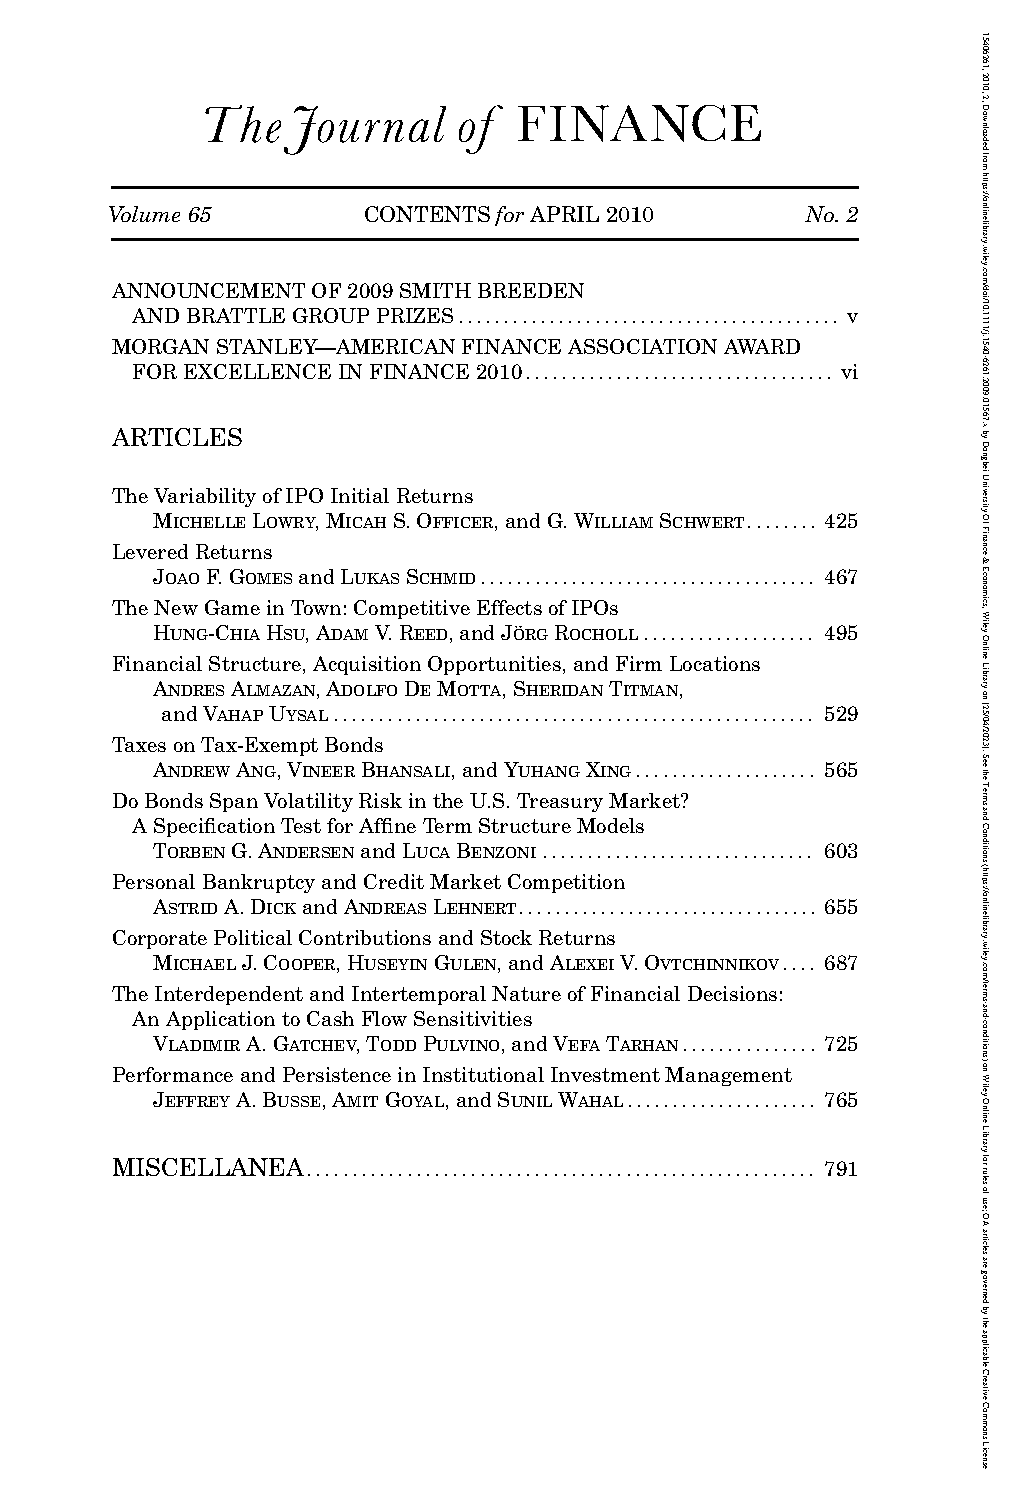
\includegraphics[height=0.7\textheight]{Files/Front}
	\end{figure}
	\begin{center}
		\footnotesize \textit{Hou, Mo, Xue, Zhang.\ \textbf{The Investment CAPM} (Cambridge University Press, 2025) --- the long-form statement of the program.}
	\end{center}
\end{frame}

\begin{frame}{The Q Camp's Tally Against Anomalies}
	\begin{figure}
		\centering
		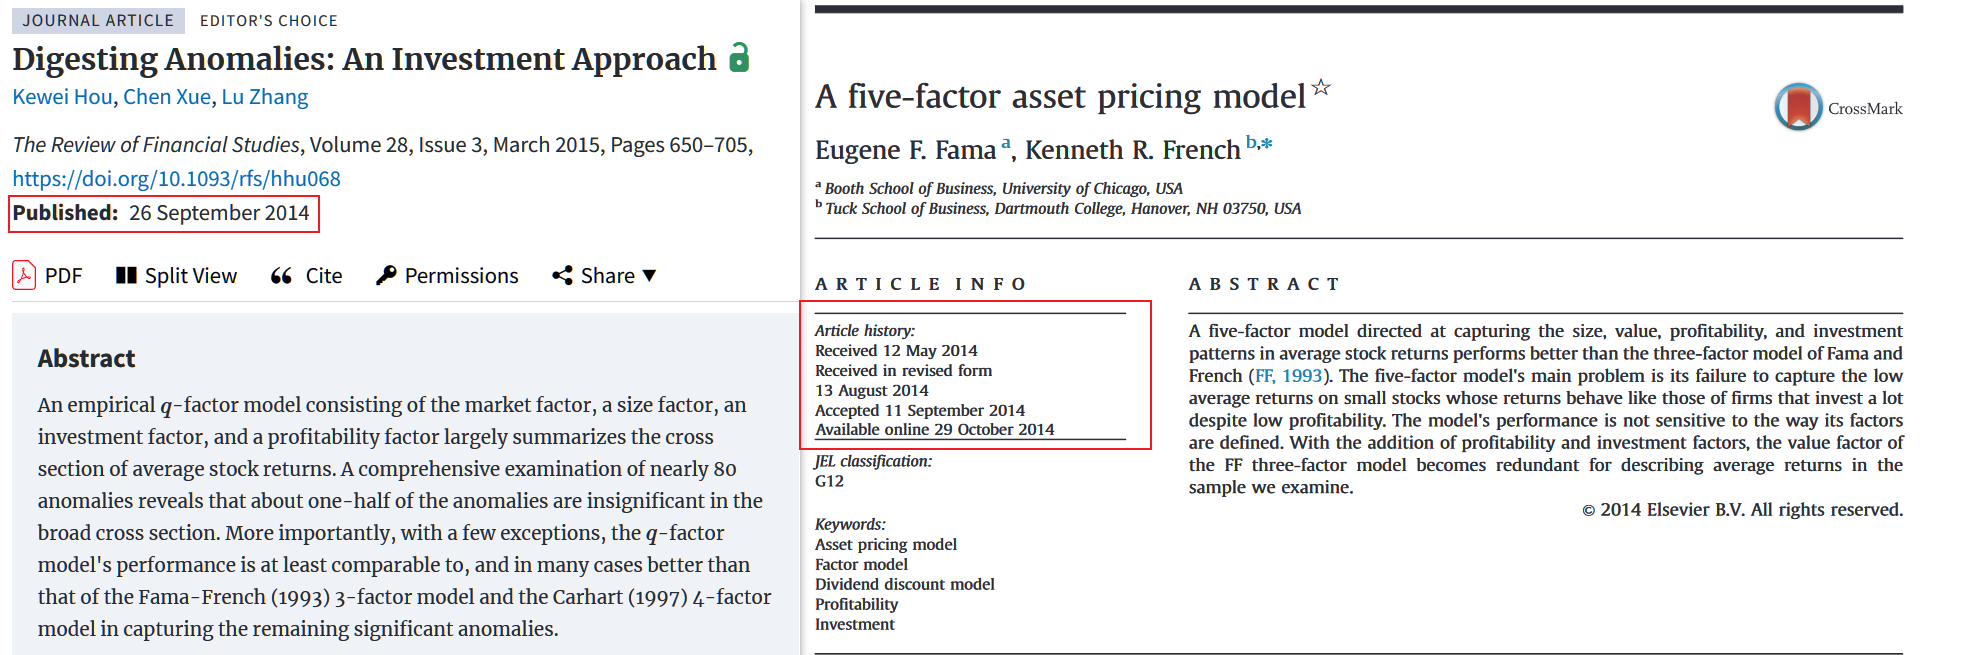
\includegraphics[width=1.0\linewidth]{Files/pk.png}
	\end{figure}
\end{frame}

% ---------------------------------------------------------
% Closing — quiet vindication
% ---------------------------------------------------------
\begin{frame}[allowframebreaks]{Closing the Showdown: A Quiet Vindication}
	\textbf{Two thoughts to hold at once:}
	\begin{enumerate}
		\item The \textit{q}-factor model is structurally cleaner: factors emerge from the firm's FOC, not from an accounting identity.
		\item FF5/FF6 remain the empirical workhorse: more flexible, easier to extend, and overwhelmingly more cited (FF5 citations $\gg$ HXZ citations on Google Scholar).
	\end{enumerate}
	\vspace{6pt}
	\textbf{Quiet signs the tide is shifting:}
	\begin{itemize}
		\item John Cochrane (Fama's son-in-law) still hosts the pre-revision Chen--Zhang manuscript on his \textit{Empirical Asset Pricing} course site under ``Production-based methods.'' \textit{Even inside the Fama family, the original paper is not erased.}
		\item HMXZ (2019) won \textit{Review of Finance}'s best paper prize.
		\item $q^{5}$ (HMXZ 2021) is, on the broadest anomaly samples available, the best-performing factor model on the market.
	\end{itemize}
	\framebreak
	\begin{block}{Preview of Lecture 07}
		The bilateral FF--HXZ fight is just one front. Once you zoom out, the literature is a \textbf{Factor Zoo}, and zoos breed \textbf{Factor Wars}: \href{https://doi.org/10.1093/rfs/hhv059}{\textcolor{blue}{Harvey--Liu--Zhu (2016)}} document 316 factors; \href{https://doi.org/10.1093/rfs/hhy131}{\textcolor{blue}{Hou--Xue--Zhang (2020)}} fail to replicate most anomalies; \href{https://doi.org/10.1111/jofi.12883}{\textcolor{blue}{Feng--Giglio--Xiu (2020)}} build a formal selection rule. The next lecture organizes the war into four battlefields.
	\end{block}
\end{frame}

\end{document}
